\documentclass[openany]{book}
\usepackage{lmodern}
\usepackage{setspace}
\setstretch{1.25}
\usepackage{amssymb,amsmath}
\usepackage{ifxetex,ifluatex}
\usepackage{fixltx2e} % provides \textsubscript
\ifnum 0\ifxetex 1\fi\ifluatex 1\fi=0 % if pdftex
  \usepackage[T1]{fontenc}
  \usepackage[utf8]{inputenc}
\else % if luatex or xelatex
  \ifxetex
    \usepackage{mathspec}
  \else
    \usepackage{fontspec}
  \fi
  \defaultfontfeatures{Ligatures=TeX,Scale=MatchLowercase}
\fi
% use upquote if available, for straight quotes in verbatim environments
\IfFileExists{upquote.sty}{\usepackage{upquote}}{}
% use microtype if available
\IfFileExists{microtype.sty}{%
\usepackage{microtype}
\UseMicrotypeSet[protrusion]{basicmath} % disable protrusion for tt fonts
}{}
\usepackage[left=4cm, right=3cm, top=2.5cm, bottom=2.5cm]{geometry}
\usepackage{hyperref}
\hypersetup{unicode=true,
            pdftitle={GDB\_DataReview ArcMap Toolbox Tutorials},
            pdfauthor={Steven C. Gonzalez \& Marie C. Cline; Air Force Civil Engineering Center (AFCEC); Geospatial Integration Office (GIO)},
            pdfborder={0 0 0},
            breaklinks=true}
\urlstyle{same}  % don't use monospace font for urls
\usepackage{natbib}
\bibliographystyle{apalike}
\usepackage{longtable,booktabs}
\usepackage{graphicx,grffile}
\makeatletter
\def\maxwidth{\ifdim\Gin@nat@width>\linewidth\linewidth\else\Gin@nat@width\fi}
\def\maxheight{\ifdim\Gin@nat@height>\textheight\textheight\else\Gin@nat@height\fi}
\makeatother
% Scale images if necessary, so that they will not overflow the page
% margins by default, and it is still possible to overwrite the defaults
% using explicit options in \includegraphics[width, height, ...]{}
\setkeys{Gin}{width=\maxwidth,height=\maxheight,keepaspectratio}
\IfFileExists{parskip.sty}{%
\usepackage{parskip}
}{% else
\setlength{\parindent}{0pt}
\setlength{\parskip}{6pt plus 2pt minus 1pt}
}
\setlength{\emergencystretch}{3em}  % prevent overfull lines
\providecommand{\tightlist}{%
  \setlength{\itemsep}{0pt}\setlength{\parskip}{0pt}}
\setcounter{secnumdepth}{5}
% Redefines (sub)paragraphs to behave more like sections
\ifx\paragraph\undefined\else
\let\oldparagraph\paragraph
\renewcommand{\paragraph}[1]{\oldparagraph{#1}\mbox{}}
\fi
\ifx\subparagraph\undefined\else
\let\oldsubparagraph\subparagraph
\renewcommand{\subparagraph}[1]{\oldsubparagraph{#1}\mbox{}}
\fi

%%% Use protect on footnotes to avoid problems with footnotes in titles
\let\rmarkdownfootnote\footnote%
\def\footnote{\protect\rmarkdownfootnote}

%%% Change title format to be more compact
\usepackage{titling}

% Create subtitle command for use in maketitle
\newcommand{\subtitle}[1]{
  \posttitle{
    \begin{center}\large#1\end{center}
    }
}

\setlength{\droptitle}{-2em}
  \title{GDB\_DataReview ArcMap Toolbox Tutorials}
  \pretitle{\vspace{\droptitle}\centering\huge}
  \posttitle{\par}
  \author{Steven C. Gonzalez \& Marie C. Cline \\ Air Force Civil Engineering Center (AFCEC) \\ Geospatial Integration Office (GIO)}
  \preauthor{\centering\large\emph}
  \postauthor{\par}
  \predate{\centering\large\emph}
  \postdate{\par}
  \date{2018-05-11}

\usepackage{booktabs}
\usepackage{graphics}
\usepackage{graphicx}
\usepackage {hyperref}
\hypersetup{linktocpage}
\hypersetup {colorlinks = true,linkcolor = blue, urlcolor = blue}
\usepackage{booktabs}
\usepackage{longtable}
\usepackage{array}
\usepackage{multirow}
\usepackage{wrapfig}
\usepackage{float}
\usepackage{colortbl}
\usepackage{framed}
\usepackage{tcolorbox}
\usepackage{fullwidth}
\usepackage{pdflscape}
\usepackage{xcolor}
\usepackage{tabu}
\usepackage{threeparttable}
\usepackage[framemethod=default]{mdframed}
\usepackage{fontspec}
\usepackage[normalem]{ulem}
\raggedbottom 
\usepackage{makeidx}
\makeindex
\frontmatter

\definecolor{shadecolor}{RGB}{248,248,248}

\newenvironment{changemargin}[2]{%
\begin{list}{}{%
\setlength{\topsep}{10pt}%
\setlength{\leftmargin}{#1}%
\setlength{\rightmargin}{#2}%
\setlength{\listparindent}{\parindent}%
\setlength{\itemindent}{\parindent}%
\setlength{\parsep}{\parskip}%
}%
\item[]
\begin{mdframed}[backgroundcolor=shadecolor]
}
{\end{mdframed}\end{list}}


\newenvironment{warnp}{\begin{changemargin}{+2cm}{+2cm}}{\end{changemargin}}


\newenvironment{warnh1}{ 
\LARGE
\bfseries
\begin{center}
}
{
\end{center}

}

\usepackage{amsthm}
\newtheorem{theorem}{Theorem}[chapter]
\newtheorem{lemma}{Lemma}[chapter]
\newtheorem{corollary}{Corollary}[chapter]
\newtheorem{proposition}{Proposition}[chapter]
\newtheorem{conjecture}{Conjecture}[chapter]
\theoremstyle{definition}
\newtheorem{definition}{Definition}[chapter]
\theoremstyle{definition}
\newtheorem{example}{Example}[chapter]
\theoremstyle{definition}
\newtheorem{exercise}{Exercise}[chapter]
\theoremstyle{remark}
\newtheorem*{remark}{Remark}
\newtheorem*{solution}{Solution}
\let\BeginKnitrBlock\begin \let\EndKnitrBlock\end
\begin{document}
\maketitle

{
\setcounter{tocdepth}{0}
\tableofcontents
}
\mainmatter

\chapter{Toolbox Overview}\label{overview}

This document gives an overview of how to use the GDB\_DataReview ArcMap
Toolbox.

The GDB\_DataReview ArcMap Toolbox provides numerous Python script tools
to expedite the review of geodatabases in comparison with a template
geodatabase model. This toolbox was developed to aid Air Force (AF)
installations in maintaining geospatial data in compliance with the
current Air Force Data Model (GeoBase 3.1.0.1) developed under the
\href{https://www.sdsfieonline.org/Components/USAF}{AF GeoBase mission}.

The GeoBase 3.1.0.1 data model is based upon the
\href{https://www.sdsfieonline.org/}{Spatial Data Standards for
Facilities, Infrastructure, and Environment (SDSFIE)} SDSFIE-V 3.1 Gold
model, which complies with the Department of Defense Instruction (DoDI)
8130.01, \emph{Installation Geospatial Information and Service}
(IGI\&S), but allows some greater flexibility within the program to aid
the AF mission. As part of the IGI\&S program, this toolbox also aids in
standardizing methods to adhere to the Fiscal Year 2017 CIP data call
required by DoDI 8130.01.

The GDB\_DataReview Toolbox provides methods to:

\begin{itemize}
\tightlist
\item
  Update feature class data using both
  \protect\hyperlink{joinCalc}{tabular} and
  \protect\hyperlink{spatjoinCalc}{spatial} joins,
\item
  Find \protect\hyperlink{dupGeom}{duplicate geometries}, delete
  \protect\hyperlink{dupFeats}{duplicate features}, and
  \protect\hyperlink{chkGeom}{check/repair} feature geometries,
\item
  Standardize \protect\hyperlink{std3}{road prefixes, names and
  suffixes} or \protect\hyperlink{stdAdd1}{building addresses},
\item
  \protect\hyperlink{indtSearch}{Search for} and
  \protect\hyperlink{summIndt}{summarize} indeterminant and missing data
  in a geodatabase when compared with a template geodatabase
\item
  Batch \protect\hyperlink{exMeta}{exporting} and
  \protect\hyperlink{imMeta}{importing} geodatabase metadata
\end{itemize}

\chapter{Opening the Toolbox}\label{opening-the-toolbox}

In order to access this toolbox, open ArcCatalog (or the ArcCatalog
window within ArcMap). Within the `Catalog Tree' windowpane in
ArcCatalog, click the Folder Connections folder and navigate to the
location of the toolbox. You may need to add a folder connection by
right clicking `Folder Connections' and clicking `Connect to Folder.'
Then navigate to the folder with the toolbox within the newly connected
folder. Then, you can click the plus sign by the toolbox to view the
tools within it (Fig. \ref{fig:opentoolbox}).

\begin{figure}[H]

{\centering 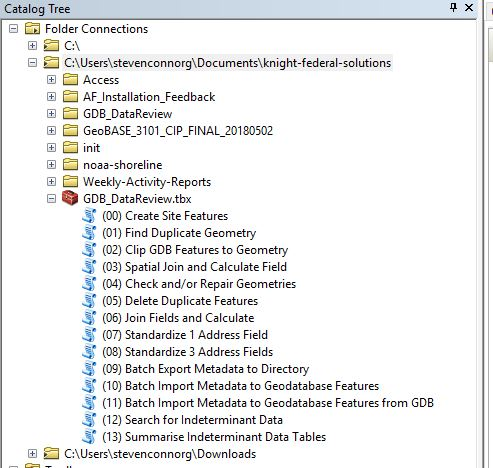
\includegraphics[width=2.57in,]{figures/opentoolbox} 

}

\caption{Opening the Create Site Data tool}\label{fig:opentoolbox}
\end{figure}

\pagebreak
\printindex

\chapter{Create Site Data}\label{siteData}

\section{Overview}\label{overview}

The Create Site Data tool allows users to use the Cadastre dataset's
Installation\_A, Site\_A, and Site\_P feature classes to populate and
update site data as needed.

This tool compares the geometry of Installation\_A data (required to be
populated) to Site\_A data and populates features where needed. Upon the
update of Site\_A, points are created in Site\_P for each feature in
Site\_A if they do not exist.

The user has the option to bypass the geometry compare between
Installation\_A and Site\_A. When bypassed, no features are added to
Site\_A and site points are created using data that already exists in
Site\_A.

\section{Parameters}\label{parameters}

The tool has 3 parameters:

\begin{enumerate}
\def\labelenumi{\arabic{enumi}.}
\tightlist
\item
  \textbf{Input\_Geodatabase (data type: Workspace)} - This parameter
  must be the path of the input geodatabase to search Feature Datasets'
  Feature Class features for duplicate features.\\
\item
  \textbf{Bypass Installation\_A and Site\_A Geometry Compare (data
  type: Boolean)} - This parameter is a check box that is unchecked by
  default. If the user checks the box, the geometry compare between
  Installation\_A and Site\_A will be bypassed.
\item
  \textbf{Installation\_A \& Site\_A Geometry Compare Type (data type:
  String Value List)} - How do you want to limit the spatial join? By
  default, this parameter is set to ``HAVE THEIR CENTER IN,'' in order
  to only update target features that have their center in the source
  features. This parameter may be changed to any of the following
  values, as specified in the
  \href{http://desktop.arcgis.com/en/arcmap/latest/tools/data-management-toolbox/select-layer-by-location.htm}{SelectByLocation\_management
  tool documentation}:

  \begin{itemize}
  \tightlist
  \item
    \emph{INTERSECT} ---The features in the input layer will be selected
    if they intersect a selecting feature. This is the default.\\
  \item
    \emph{INTERSECT\_3D} ---The features in the input layer will be
    selected if they intersect a selecting feature in three-dimensional
    space (x, y, and z).\\
  \item
    \emph{WITHIN\_A\_DISTANCE} ---The features in the input layer will
    be selected if they are within a specified distance of a selecting
    feature. Specify a distance in the Search Distance parameter.\\
  \item
    \emph{WITHIN\_A\_DISTANCE\_3D} ---The features in the input layer
    will be selected if they are within a specified distance of a
    selecting feature in three-dimensional space. Specify a distance in
    the Search Distance parameter.\\
  \item
    \emph{WITHIN\_A\_DISTANCE\_GEODESIC} ---The features in the input
    layer will be selected if they are within a specified distance of a
    selecting feature. Distance between features will be calculated
    using a geodesic method which takes into account the curvature of
    the earth and correctly deals with data near and across the dateline
    and poles.\\
  \item
    \emph{CONTAINS} ---The features in the input layer will be selected
    if they contain a selecting feature.\\
  \item
    \emph{COMPLETELY\_CONTAINS} ---The features in the input layer will
    be selected if they completely contain a selecting feature.\\
  \item
    \emph{CONTAINS\_CLEMENTINI} ---This spatial relationship yields the
    same results as COMPLETELY\_CONTAINS with the following exception:
    if the selecting feature is entirely on the boundary of the input
    feature (no part is properly inside or outside), the feature will
    not be selected. Clementini defines the boundary polygon as the line
    separating inside and outside, the boundary of a line is defined as
    its end points, and the boundary of a point is always empty.\\
  \item
    \emph{WITHIN} ---The features in the input layer will be selected if
    they are within a selecting feature.\\
  \item
    \emph{COMPLETELY\_WITHIN} --- The features in the input layer will
    be selected if they are completely within or contained by a
    selecting feature.\\
  \item
    \emph{WITHIN\_CLEMENTINI} --- The result will be identical to WITHIN
    with the exception that if the entirety of the feature in the input
    layer is on the boundary of the feature in the selecting layer, the
    feature will not be selected. Clementini defines the boundary
    polygon as the line separating inside and outside, the boundary of a
    line is defined as its end points, and the boundary of a point is
    always empty.\\
  \item
    \emph{ARE\_IDENTICAL\_TO} --- The features in the input layer will
    be selected if they are identical (in geometry) to a selecting
    feature.
  \end{itemize}
\end{enumerate}

\section{How to Use}\label{how-to-use}

\subsection{Begin by opening the
toolbox}\label{begin-by-opening-the-toolbox}

Navigate to the location of the script toolbox, then right-click the
`Create Site Data' script tool to open (Fig. \ref{fig:csdopen}).

\begin{figure}[H]

{\centering 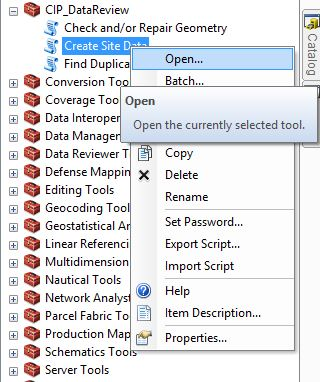
\includegraphics[width=1.67in,]{figures/csd-open} 

}

\caption{Opening the Create Site Data tool}\label{fig:csdopen}
\end{figure}

\subsection{Fill out the parameters}\label{fill-out-the-parameters}

Next, fill out the parameters for the tool. Here, we want to select the
Cadastre feature dataset for the geodatabase being processed. (Fig.
\ref{fig:csdparams}). Last, we specify where we want to output the
resulting tables, prefereably in an Installation Review geodatabase
specifically for holding CIP processing results.\\

\begin{figure}[H]

{\centering 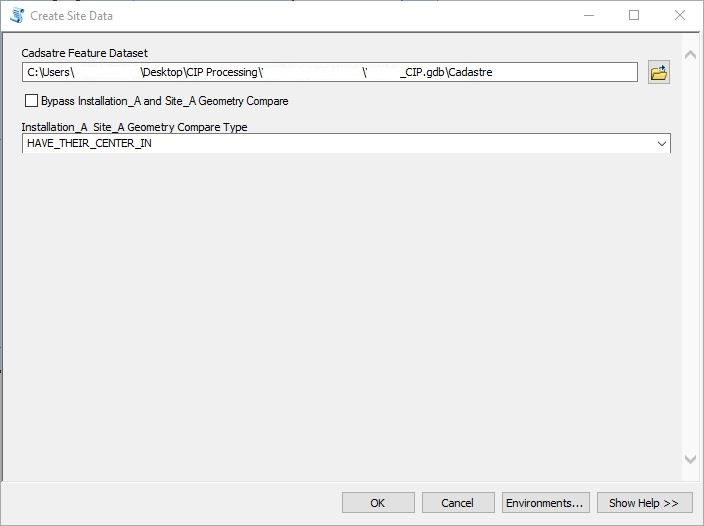
\includegraphics[width=3.67in,]{figures/csd-params} 

}

\caption{Create Site Data Tool parameters}\label{fig:csdparams}
\end{figure}

\subsection{Run the Tool and View
Results}\label{run-the-tool-and-view-results}

While the tool runs (with Background Processing disabled), we can see
messages and warnings from the tool. Warnings are provided if required
feature classes are missing or data verification from the user is
suggested. Messages include the number of features added to Site\_A and
the number of points added to Site\_P (Fig. \ref{fig:delFmessages}).
Here, we see that an Installation\_A feature exists beyond the
boundaries of the Site\_A features so 1 feature is appended to Site\_A.
Then, 8 site points were created for the empty Site\_P feature class.

\begin{figure}[H]

{\centering 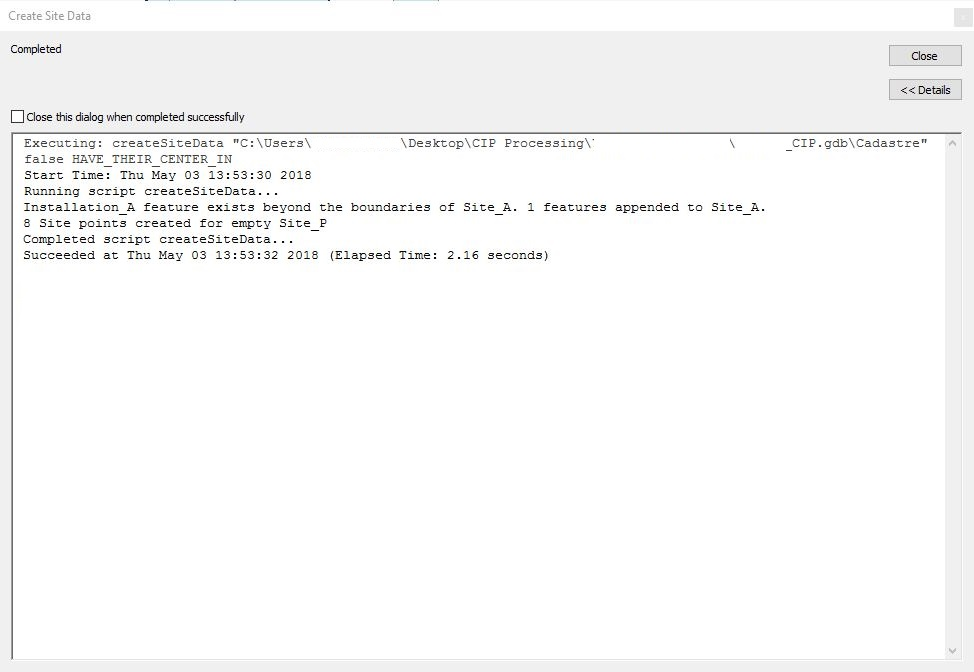
\includegraphics[width=5.07in,]{figures/csd-messages} 

}

\caption{Create Site Data tool messages}\label{fig:csdmessages}
\end{figure}

After running the tool, we can see the Site\_P and Site\_A features are
created properly, where previously missed (Fig. \ref{fig:csdbefore} \&
Fig. \ref{fig:csdafter}).

\begin{figure}[H]

{\centering 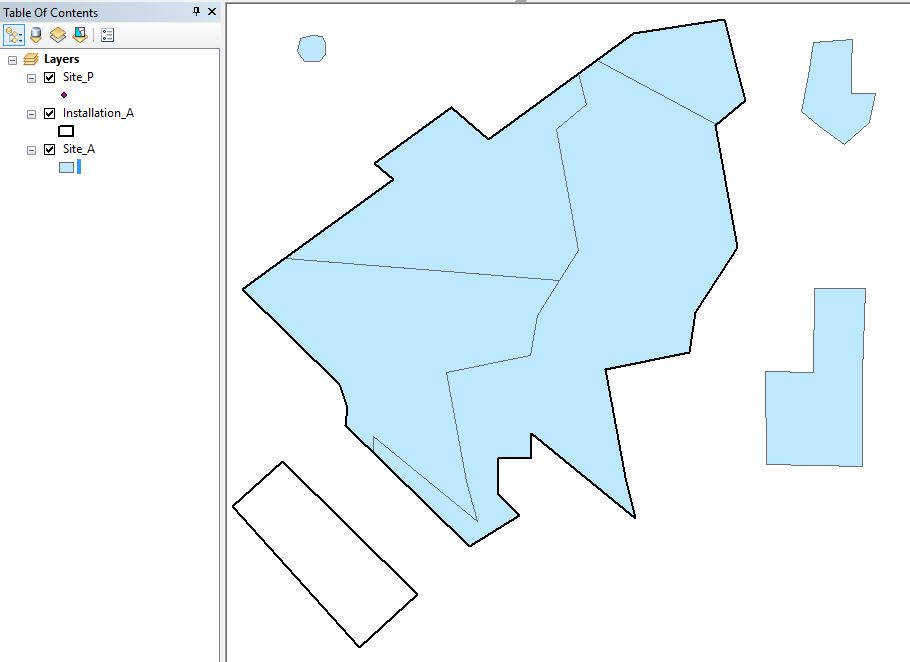
\includegraphics[width=4.74in,]{figures/csd-before} 

}

\caption{Before running the tool}\label{fig:csdbefore}
\end{figure}\begin{figure}[H]

{\centering 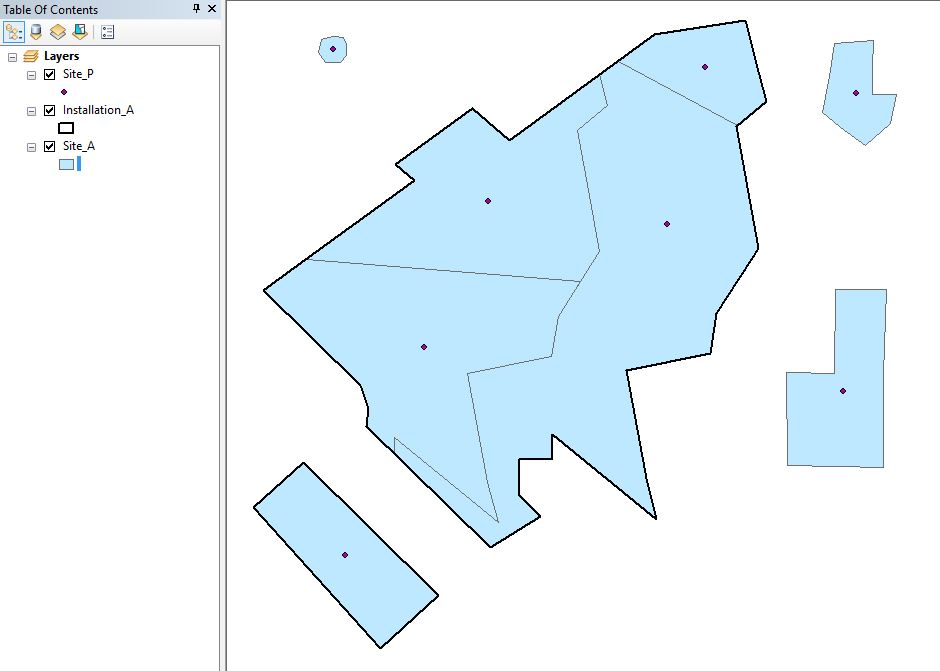
\includegraphics[width=4.9in,]{figures/csd-after} 

}

\caption{Newly created Site A and Site P features after running the tool}\label{fig:csdafter}
\end{figure}

\hypertarget{joinCalc}{\chapter{Join Fields and
Calculate}\label{joinCalc}}

\section{Overview}\label{overview-1}

The ArcGIS Python Script Tool ``Join Fields and Calculate'' may be used
to update the destination values in a target feature layer field with
the values in another table's fields using a common key (join). This
script will perform similarly as if you joined a table to a feature
class to calculate a certain field based on another field in the joined
table.

\section{Parameters}\label{parameters-1}

The tool has 8 parameters:

\begin{enumerate}
\def\labelenumi{\arabic{enumi}.}
\item
  \textbf{Transfer\_From (data type: Table View)} - Which table are do
  you want to transfer data from? This parameter must be the path to a
  table(e.g.: Comma-separated Values (.csv) file, Excel Workbook (.xlsx)
  Sheet, Esri geodatabase table, etc.). This table will act as `source'
  data.
\item
  \textbf{Using\_Join\_Field (data type: Field)} - From the source
  table, which field should be used to joinwith another feature class'
  attributes? This will provide the `key' to transfer data from the
  source table to the target table.
\item
  \textbf{Source\_Field (data type: Field)} - From the source table,
  which field's data do you want to transfer to the target table? This
  field's data will be updated in the target feature class that have
  matching fields.
\item
  \textbf{Destination\_Feature (data type: Feature Layer or Feature
  Class)} - Which feature class do you want to transfer data to? This
  parameter must be the path to a Esri Feature Class or Feature Layer.
  This table will act as `target' data source.
\item
  \textbf{Destination\_Join\_Field (data type: Field)} - From the target
  table, which field should be used to joinwith another feature class'
  attributes? This will provide the `key' to transfer data from the
  source table to the target table.
\item
  \textbf{Destination\_Field (data type: Field)} - From the target
  table, which field's data do you want to transfer from the source
  table? This field's data will be updated from the source table that
  have matching fields using the join fields provided.
\item
  \textbf{Where\_Clause (data type: String)} - How should the source
  values be filtered? Default is ``IS NOT NULL'', otherwise you will
  overwrite the target features will null values.
\item
  \textbf{Remove\_Leading\_Zeros (data type: Boolean)} - Do you want to
  remove leading zeros from the Source Join Field prior to `joining' the
  tables?
\item
  \textbf{Source RPSUID Field (data type: Field)} - Which field in the
  source table holds the Real Property Site Unique ID values? This field
  acts as a second join ``key'' to ensure that the correct Real Property
  Unique IDs are joined for each unique Site (i.e.: RPSUID).
\item
  \textbf{Update RPSUID Field (data type: Field)} - Which field in the
  Destination Feature holds the Real Property Site Unique ID values?
  This field acts as a second join ``key'' to ensure that the correct
  Real Property Unique IDs are joined for each unique Site (i.e.:
  RPSUID).
\end{enumerate}

\section{How to Use}\label{how-to-use-1}

\subsection{Begin by opening the
toolbox}\label{begin-by-opening-the-toolbox-1}

Navigate to the location of the script tool, then right-click the `Join
Fields and Calculate' script tool to open (Fig. \ref{fig:jcopen}).

\begin{figure}[H]

{\centering 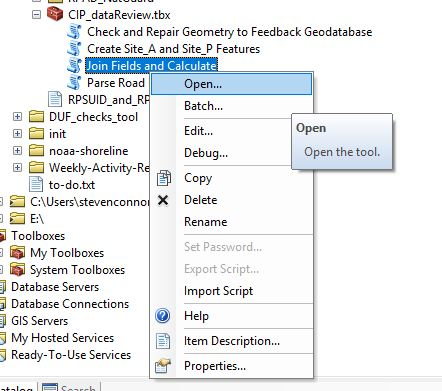
\includegraphics[width=2.3in,]{figures/joinCalcopentool} 

}

\caption{Opening the Tool}\label{fig:jcopen}
\end{figure}

\subsection{Fill out the parameters}\label{fill-out-the-parameters-1}

Next, fill out the parameters for the tool. Here, we want to transfer
the RPUID attributes (source field) from the `RPSUID\_and\_RPUID.csv'
table (transfer from) using the `FacilityNumber' join field
(Using\_Join\_Field) to the Building\_A feature layer's (Destination
Feature) `realPropertyUniqueID' field (Destination\_Field) using the
`buildingNumber' field (Destination\_Join\_Field) (Fig.
\ref{fig:jcparams}).

We also keep the default value in the `Where Clause' parameter of `IS
NOT NULL,' in order to transfer RPUID from the source table where RPUIDs
are not null, \textbf{otherwise you may overwrite the target features
will null values} (Fig. \ref{fig:jcparams}).

We noticed that the `buildingNumber' field has some leading zeros that
we want to remove the beginning of the values, so we click the ``Remove
Leading Zeros'' toggle (Fig. \ref{fig:jcparams}). If you noticed that
the `Destination Join Field' values have leading spaces, you can also
check the `Remove\_Leading\_Zeros' parameter to remove these spaces.

\begin{figure}[H]

{\centering 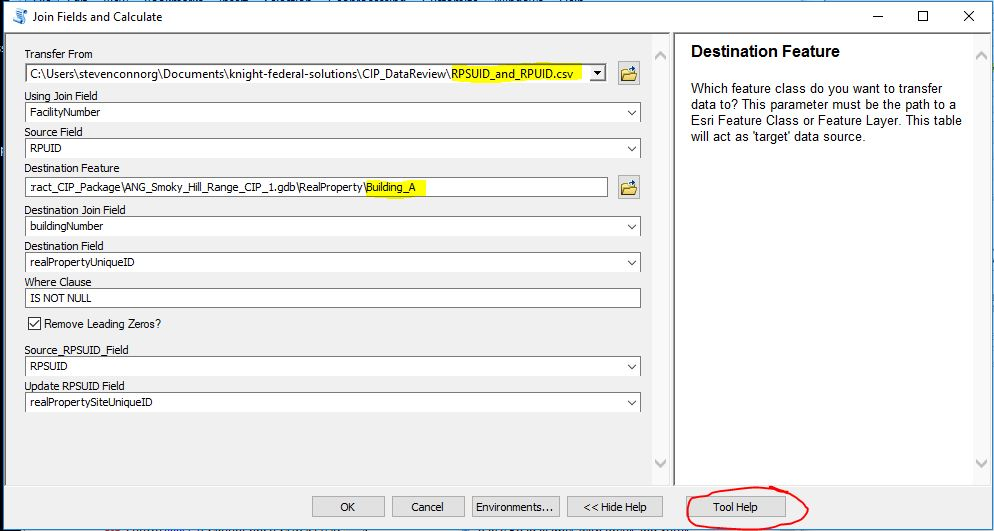
\includegraphics[width=5.18in,]{figures/joinCalc-toolparams} 

}

\caption{Tool parameters}\label{fig:jcparams}
\end{figure}

Alternatively, you may also run this tool in `batch' for multiple
features in a geodatabase or geodatabases (Fig. \ref{fig:batch}).

\begin{figure}[H]

{\centering 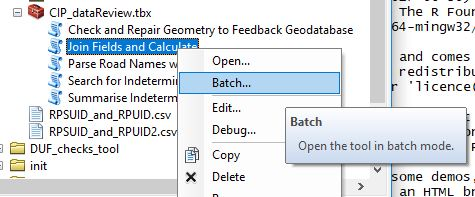
\includegraphics[width=2.47in,]{figures/joinCalc-batch} 

}

\caption{Running a tool in batch}\label{fig:batch}
\end{figure}

You may also get more information for the tool and each tool parameter
by clicking the `Tool Help' button at the bottom of the tool dialog box.

\subsection{Run the Tool and View
Results}\label{run-the-tool-and-view-results-1}

Open the destinate Feature Class and view the update destination field
values (Fig. \ref{fig:jcbefore}, Fig. \ref{fig:jcafter}).

\begin{figure}[H]

{\centering 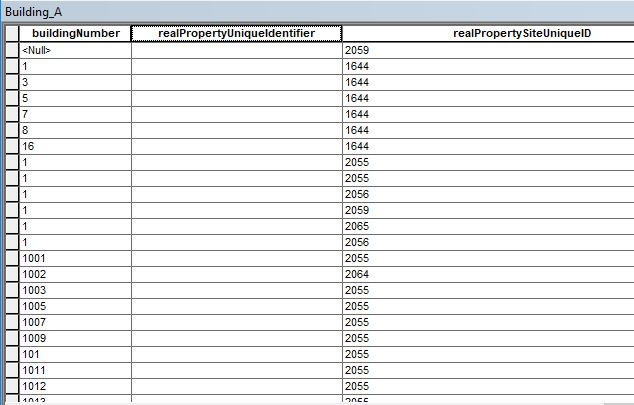
\includegraphics[width=3.3in,]{figures/joinCalc-before} 

}

\caption{Attribues before running the Join Fields and Calculate tool}\label{fig:jcbefore}
\end{figure}

\begin{figure}[H]

{\centering 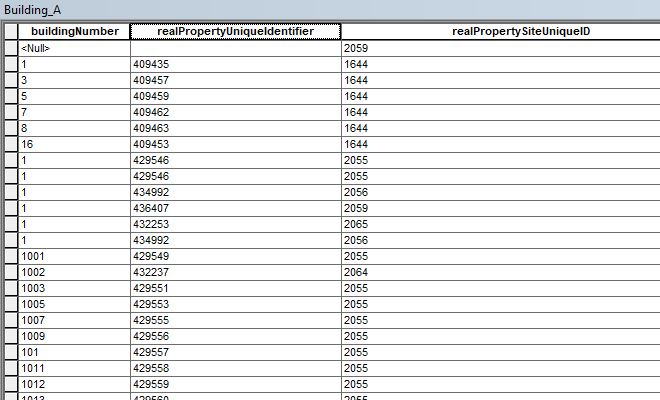
\includegraphics[width=3.44in,]{figures/joinCalc-results} 

}

\caption{Attributes after running the tool, matching against both Building Number and RPSUID to update RPUID values}\label{fig:jcafter}
\end{figure}

\hypertarget{spatjoinCalc}{\chapter{Spatial Join and
Calculate}\label{spatjoinCalc}}

\section{Overview}\label{overview-2}

This tool utilizes spatial joins to update field values in the target
Feature Classes field to equal the source Feature Class fields in a
source geodatabase. Using `wildcard' fitlers, this tool allows users to
update particular target Feature Datasets, Feature Classes, and Fields.
For the purposes of this tool within the scope of the CIP Data Review
task, target Fields are, by default, any fields that begin with
``realPropertySiteUnique,'' in order to udpate RPSUID fields called
either ``realPropertySiteUniqueIdentifier'' or
``realPropertySiteUniqueID''; however, this tool could be extended to
any number of source/target Feature Class/Field values.

\section{Parameters}\label{parameters-2}

The tool has 8 parameters:

\begin{enumerate}
\def\labelenumi{\arabic{enumi}.}
\item
  \textbf{Update Geodatabase (data type: Workspace/File Geodatabase)} -
  The path to the input geodatabase to update Feature Classes in.
\item
  \textbf{Source Feature (data type: Feature Class)} - The path to the
  source Feature Class, which will be used to update Feature Class
  fields in target Feature Classes.
\item
  \textbf{Source\_Field (data type: Field)} - The field within the
  source Feature Class used to update values in target Feature Classes.
\item
  \textbf{Target Feature Dataset Wildcard (data type: String)} - Within
  the input geodatabase, do you want to update only certain Feature
  Datasets? Use this wildcard to filter input geodatabase Feature
  Datasets. The Default is `*' for `All Feature Datasets,' but if you
  only wanted to update the Feature Classes in the `Auditory' Feature
  Dataset, set this parameter to `Auditory.' Similarly, if you only
  wanted to update Feature Classes within environmental Feature
  Datasets, set this parameter to 'environmental*`, which will loop
  through all Feature Classes within Feature Datasets that start with
  'environmental.'
\item
  \textbf{Target Feature Class Wildcard (data type: String)} - Within
  the input geodatabase, do you want to update only certain Feature
  Classes? Use this wildcard to filter input geodatabase Feature Classes
  to update. The Default is `*' for `All Feature Classes,' but if you
  only wanted to update Feature Classes called ``roadCenterline\_L'',
  set this parameter to `roadCenterline\_L.' Similarly, if you only
  wanted to update Feature Classes that begin with ``road,'' set this
  parameter to 'road*`, which will loop through all Feature Classes that
  start with 'road.'
\item
  \textbf{Target Field Wildcard (data type: String)} - This parameter is
  used to filter fields within the target Feature Classes that you want
  to update with the Source Feature Classes source Field. For the
  purposes of this tool within the scope of the CIP Data Review, this
  parameter is automatically set to ``realPropertySiteUnique*" in order
  to `catch' all RPSUID fields within the SDSFIE 3.101 data model, where
  certain fields are called ``realPropertySiteUniqueIdentifier'' and
  others are called ``realPropertySiteUniqueID.''
\item
  \textbf{Overlap Type (data type: String)} - How do you want to limit
  the spatial join? By default, this parameter is set to ``within,'' in
  order to only update target features that are completely within the
  source features. This parameter may be changed to any of the following
  values, as specified in the
  \href{http://desktop.arcgis.com/en/arcmap/latest/tools/data-management-toolbox/select-layer-by-location.htm}{SelectByLocation\_management
  tool documentation}:

  \begin{itemize}
  \tightlist
  \item
    \emph{INTERSECT} ---The features in the input layer will be selected
    if they intersect a selecting feature. This is the default.\\
  \item
    \emph{INTERSECT\_3D} ---The features in the input layer will be
    selected if they intersect a selecting feature in three-dimensional
    space (x, y, and z).\\
  \item
    \emph{WITHIN\_A\_DISTANCE} ---The features in the input layer will
    be selected if they are within a specified distance of a selecting
    feature. Specify a distance in the Search Distance parameter.\\
  \item
    \emph{WITHIN\_A\_DISTANCE\_3D} ---The features in the input layer
    will be selected if they are within a specified distance of a
    selecting feature in three-dimensional space. Specify a distance in
    the Search Distance parameter.\\
  \item
    \emph{WITHIN\_A\_DISTANCE\_GEODESIC} ---The features in the input
    layer will be selected if they are within a specified distance of a
    selecting feature. Distance between features will be calculated
    using a geodesic method which takes into account the curvature of
    the earth and correctly deals with data near and across the dateline
    and poles.\\
  \item
    \emph{CONTAINS} ---The features in the input layer will be selected
    if they contain a selecting feature.\\
  \item
    \emph{COMPLETELY\_CONTAINS} ---The features in the input layer will
    be selected if they completely contain a selecting feature.\\
  \item
    \emph{CONTAINS\_CLEMENTINI} ---This spatial relationship yields the
    same results as COMPLETELY\_CONTAINS with the following exception:
    if the selecting feature is entirely on the boundary of the input
    feature (no part is properly inside or outside), the feature will
    not be selected. Clementini defines the boundary polygon as the line
    separating inside and outside, the boundary of a line is defined as
    its end points, and the boundary of a point is always empty.\\
  \item
    \emph{WITHIN} ---The features in the input layer will be selected if
    they are within a selecting feature.\\
  \item
    \emph{COMPLETELY\_WITHIN} --- The features in the input layer will
    be selected if they are completely within or contained by a
    selecting feature.\\
  \item
    \emph{WITHIN\_CLEMENTINI} --- The result will be identical to WITHIN
    with the exception that if the entirety of the feature in the input
    layer is on the boundary of the feature in the selecting layer, the
    feature will not be selected. Clementini defines the boundary
    polygon as the line separating inside and outside, the boundary of a
    line is defined as its end points, and the boundary of a point is
    always empty.\\
  \item
    \emph{ARE\_IDENTICAL\_TO} --- The features in the input layer will
    be selected if they are identical (in geometry) to a selecting
    feature.\\
  \item
    \emph{BOUNDARY\_TOUCHES} --- The features in the input layer will be
    selected if they have a boundary that touches a selecting feature.
    When the inputs features are lines or polygons, the boundary of the
    input feature can only touch the boundary of the selecting feature,
    and no part of the input feature can cross the boundary of the
    selecting feature.\\
  \item
    \emph{SHARE\_A\_LINE\_SEGMENT\_WITH} --- The features in the input
    layer will be selected if they share a line segment with a selecting
    feature. The input and selecting features must be line or polygon.\\
  \item
    \emph{CROSSED\_BY\_THE\_OUTLINE\_OF} --- The features in the input
    layer will be selected if they are crossed by the outline of a
    selecting feature. The input and selecting features must be lines or
    polygons. If polygons are used for the input or selecting layer, the
    polygon's boundary (line) will be used. Lines that cross at a point
    will be selected, not lines that share a line segment.\\
  \item
    \emph{HAVE\_THEIR\_CENTER\_IN} --- The features in the input layer
    will be selected if their center falls within a selecting feature.
    The center of the feature is calculated as follows: for polygon and
    multipoint, the geometry's centroid is used, and for line input, the
    geometry's midpoint is used.\\
  \end{itemize}
\item
  \textbf{Search Distance (data type: String)} - If the overlap type
  parameter is equal to ``WITHIN\_A\_DISTANCE\_GEODESIC'',
  ``WITHIN\_A\_DISTANCE'', ``WITHIN\_A\_DISTANCE\_3D'', ``INTERSECT'',
  ``INTERSECT\_3D'', ``HAVE\_THEIR\_CENTER\_IN'', ``CONTAINS'', or
  ``WITHIN'', you must provide a search distance.
\end{enumerate}

\section{How to Use}\label{how-to-use-2}

\subsection{Begin by opening the
toolbox}\label{begin-by-opening-the-toolbox-2}

Navigate to the location of the script tool, then right-click the
`Calculate Feature RPSUIDs from Overlapping Polygon' script tool to open
(Fig. \ref{fig:sjcopentool}).

\begin{figure}[H]

\hfill{}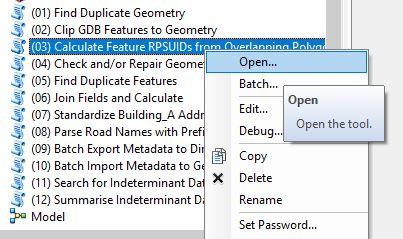
\includegraphics[width=2.1in,]{figures/spatjoinCalcopentool} 

\caption{Opening the toolbox}\label{fig:sjcopentool}
\end{figure}

\subsection{Fill out the parameters}\label{fill-out-the-parameters-2}

For this demostration, we want to update missing RPSUID values for 2
features in the Site\_P Feature Class using RPSUID values from Site\_A
features that contain Site\_P features \ref{fig:sjcbefore}).

\begin{figure}[H]

{\centering 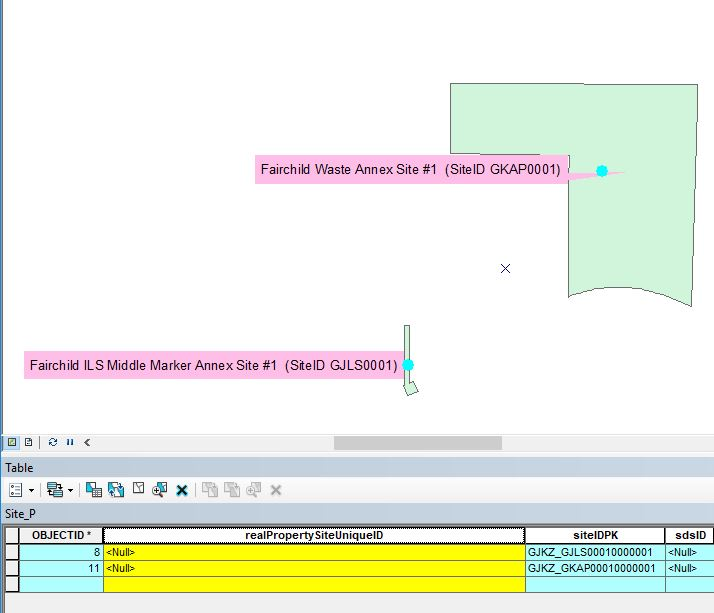
\includegraphics[width=3.72in,]{figures/spatjoinCalc-before} 

}

\caption{Missing RPSUID attributes for Site Point features}\label{fig:sjcbefore}
\end{figure}

Next, fill out the parameters for the tool. Here, we want to transfer
the RPSUID attributes (Source Field) from the Site\_A Feature Class in
the Cadastre Feature Dataset (Fig. \ref{fig:sjcparams}).

\begin{figure}[H]

{\centering 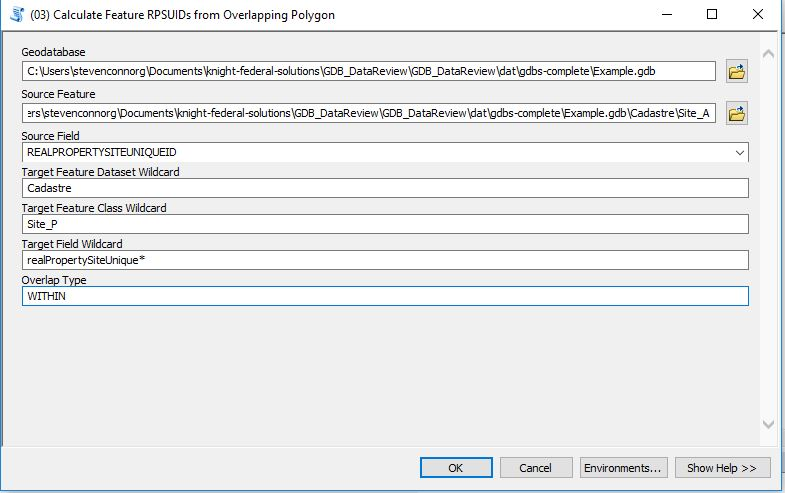
\includegraphics[width=4.09in,]{figures/spatjoinCalc-toolparams} 

}

\caption{Tool parameters}\label{fig:sjcparams}
\end{figure}

Since we only want to update the Site\_P features within the Cadastre
Feature Dataset, we change the default value for the Target Feature
Dataset Wildcard to ``Cadastre,'' since we know that the Site\_P Feature
Class is only found within the Cadastre Feature Dataset. Further, we
change the default value of the Target Feature Class Wildcard parameters
to ``Site\_P'' in order to only update Site\_P features within the
Cadastre Dataset. Since we know that the RPSUID field names within all
Feature Classes in the data model begin with `realPropertySiteUnique',
we can keep the default value for the Target Field Wildcard parameter in
order to update the realPropertySiteUniqueID field in Site\_P features
with with the Source Field in the Source Feature Class. For the purposes
of this demostration, we keep the default value for the Overlap Type
parameter to ``WITHIN,'' in order to update the fields that begin with
``realPropertySiteUnique'' for features that are \emph{within} each
Source Feature Class feature. You may also get more information for the
tool and each tool parameter by clicking the `Tool Help' button at the
bottom of the tool dialog box.

\section{Run the Tool and View
Results}\label{run-the-tool-and-view-results-2}

If running the tool with Background Processessing disabled, we can see
which RPSUIDs are being updated (Fig. \ref{fig:sjcmessages}).

\begin{figure}[H]

{\centering 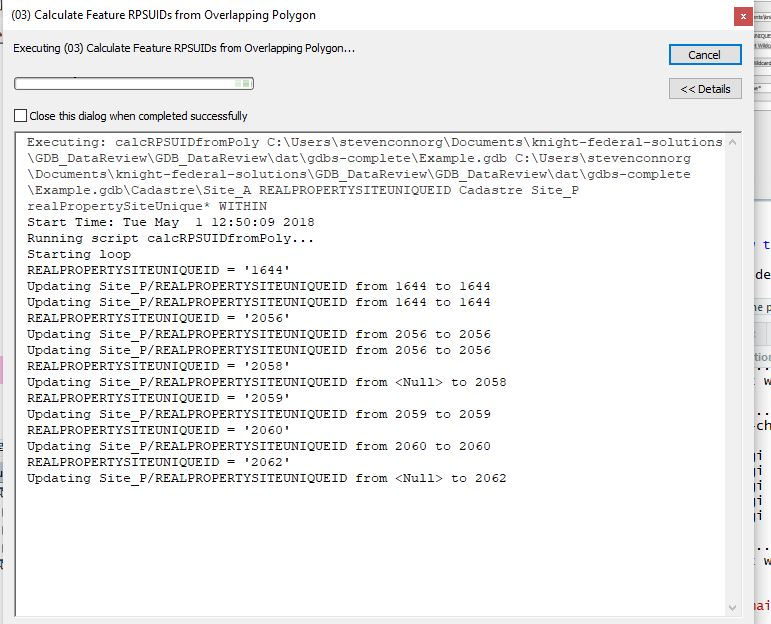
\includegraphics[width=4.02in,]{figures/spatjoinCalc-toolmessages} 

}

\caption{Tool parameters}\label{fig:sjcmessages}
\end{figure}

After the tool has run, we see that the 2 Site\_P features with missing
RPSUID values are updated accordingly \ref{fig:sjcafter}).

\begin{figure}[H]

{\centering 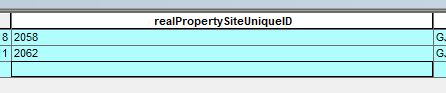
\includegraphics[width=2.32in,]{figures/spatjoinCalc-after} 

}

\caption{AFter running the tool, new Site A feaures and new Site P features are created.}\label{fig:sjcafter}
\end{figure}

\hypertarget{dupGeom}{\chapter{Find Duplicate Geometry}\label{dupGeom}}

\section{Overview}\label{overview-3}

The Find Duplicate Geometry tool allows users to search an entire
geodatabase's Feature Classes within Feature Datasets for features with
duplicate geometries. This tool loops through each Feature Dataset's
Feature Class features and searches for duplicate geometries.

All features with duplicate geometries are written to the output .csv
file, as specified, and describes the Feature Dataset and Feature Class
with duplicate geometries, the OBJECTIDs of the duplicate geometries,
and a summary, which gives the count of duplicate geometries spread over
unique geometries. Further, this tool creates layer files for each
Feature Class' duplicate features, \emph{allowing users to edit their
geodatabase directory from a temporary, filtered layer of only duplicate
features to be evaluated further, instead of arbitrarily deleting
duplicated features without further consideration.}

\section{Parameters}\label{parameters-3}

The tool has 5 parameters:

\begin{enumerate}
\def\labelenumi{\arabic{enumi}.}
\tightlist
\item
  \textbf{Input\_Geodatabase (data type: Workspace)} - This parameter
  must be the path of the input geodatabase to search Feature Datasets'
  Feature Class features for duplicate geometries.\\
\item
  \textbf{XY\_Tolerance (data type: String)} - The XY\_Tolerance
  parameter will be applied to each vertex when evaluating if there is
  an identical vertex in another entity, and must be input in the same
  units as the the source geodatabase's coordinate reference system
  (CRS).
\item
  \textbf{Z\_Tolerance (data type: String)} - The Z\_Tolerance parameter
  will be applied to each vertex when evaluating if there is an
  identical vertex in another entity with regard to elevation, and must
  be input in the same units as the the source geodatabase's coordinate
  reference system (CRS).
\item
  \textbf{Output\_CSV (data type: File)} - The path to the output
  Duplicate\_Geometry\_Summary .xlsx/.csv file.
\item
  \textbf{Output\_Layers\_Directory (data type: Folder)} - The path to
  the directory/folder to store layer files with duplicate geometries.
\end{enumerate}

\section{How to Use}\label{how-to-use-3}

\subsection{Begin by opening the
toolbox}\label{begin-by-opening-the-toolbox-3}

Navigate to the location of the script toolbox, then right-click the
`Find Duplicate Geometry' script tool to open (Fig. \ref{fig:dupGopen}).

\begin{figure}[H]

{\centering 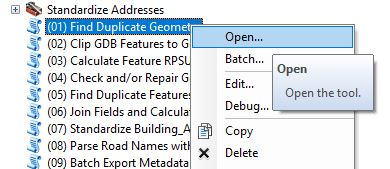
\includegraphics[width=2.03in,]{figures/dupG-opentool} 

}

\caption{Opening the Find Duplicate Geometries tool}\label{fig:dupGopen}
\end{figure}

\subsection{Fill out the parameters}\label{fill-out-the-parameters-3}

Next, fill out the parameters for the tool. Here, we want to search all
Feature Classes within Feature Datasets in the Example.gdb for duplicate
geometries using the default XY Tolerance and Z Tolerance values of `0'
(Fig. \ref{fig:dupGparams}). We specify that we want the Duplicate
Geometry Summary to be written to a Comma-separated Values (.csv) file
called `test.csv.' Further, we specify that we want all the duplicate
Feature Class feature layers to be saved to the Output Layers Directory
`layer.'

\begin{figure}[H]

{\centering 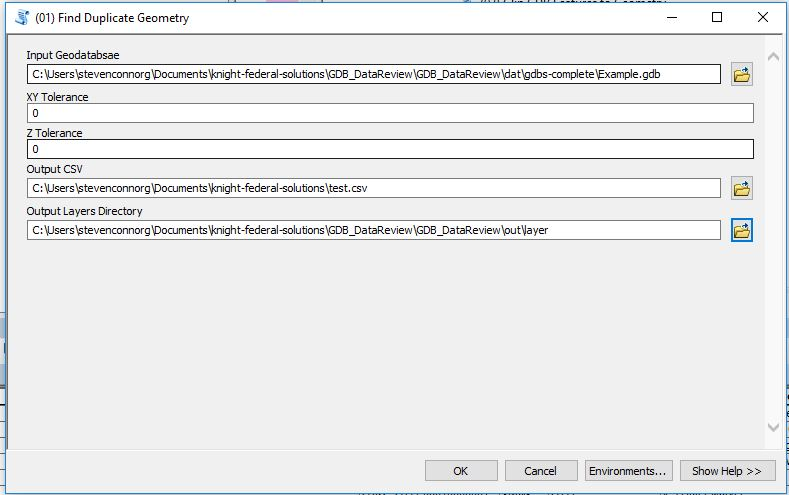
\includegraphics[width=4.11in,]{figures/dupG-params} 

}

\caption{Find Duplicate Geometries parameters}\label{fig:dupGparams}
\end{figure}

\section{Run the Tool and View
Results}\label{run-the-tool-and-view-results-3}

While the tool runs (with Background Processing disabled), we can see
the messages from the tool, showing how many duplicate features are
found for each Feature Class (Fig. \ref{fig:dupGmessages}).

\begin{figure}[H]

{\centering 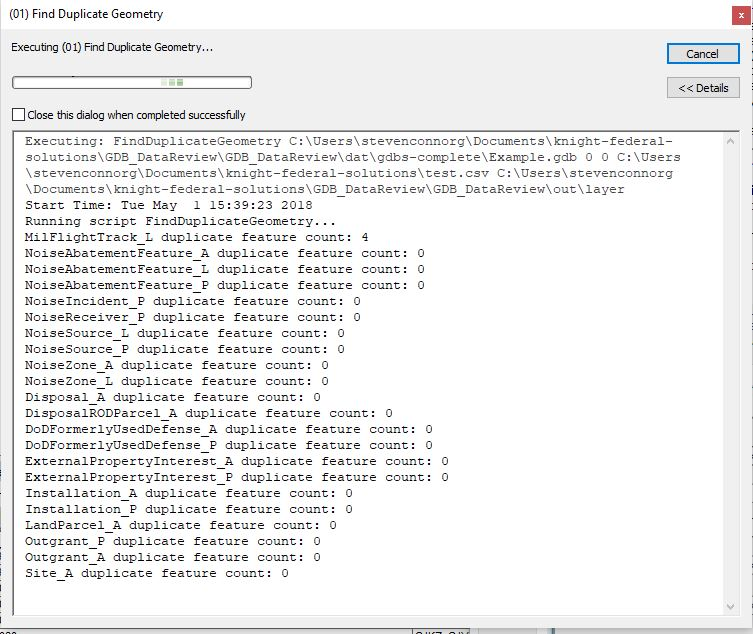
\includegraphics[width=3.92in,]{figures/dupG-messages} 

}

\caption{Messages from the Find Duplicate Geometries tool}\label{fig:dupGmessages}
\end{figure}

After the tool has run, we can open the output .csv we specified in the
tool parameters to examine which Feature Classes have duplicated
geometries . For example, we find that the EnvRestorSampLoc\_P Feature
Class within the environmentalRestoration Feature Dataset has 17 total
duplicates spread across 7 unique geometries (Fig. \ref{fig:dupGcsv}).

\begin{figure}[H]

{\centering 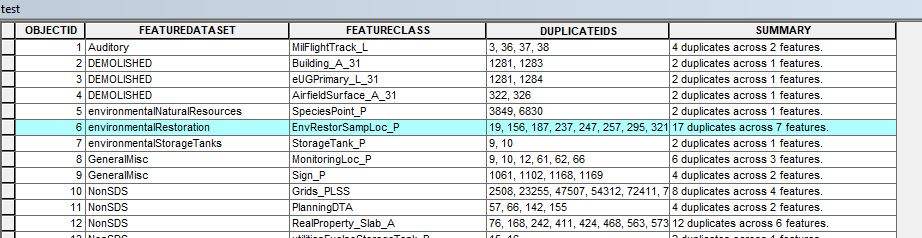
\includegraphics[width=4.8in,]{figures/dupG-csv} 

}

\caption{Find Duplicate Geometries parameters}\label{fig:dupGcsv}
\end{figure}

Navigating to the output layer directory we specified in the tool, we
find layer files with duplicate features for each Feature Class (Fig.
\ref{fig:dupGlays}).

\begin{figure}[H]

{\centering 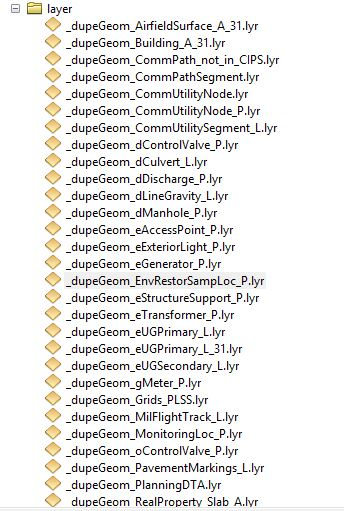
\includegraphics[width=1.79in,]{figures/dupG-lays} 

}

\caption{Find Duplicate Geometries parameters}\label{fig:dupGlays}
\end{figure}

After pulling in the \_dupeGeom\_EnvRestorSampLoc\_P layer file, we can
zoom to a feature and select the features at that location to examine
the duplicate features at that location (Fig. \ref{fig:layFeats}).

\begin{figure}[H]

{\centering 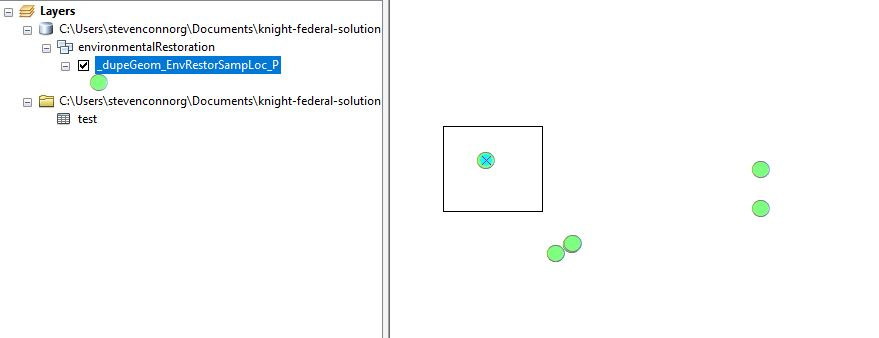
\includegraphics[width=4.58in,]{figures/dupG-layFeats} 

}

\caption{The features with duplicated geometries}\label{fig:layFeats}
\end{figure}

Then, we can view the Attribute Table for the selected features to
examine which feature we should amend or delete (Fig.
\ref{fig:layAtts}). Here, we find that the attributes are exactly the
same for the first duplicated geometry, and so we should probably delete
one of these features. Editing the layer files directly will update the
associated Feature Classes in the original geodatabase.

\begin{figure}[H]

{\centering 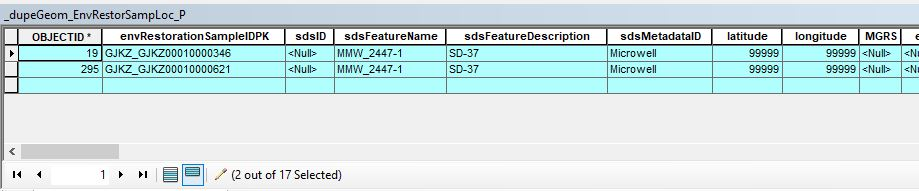
\includegraphics[width=4.79in,]{figures/dupG-layAtts} 

}

\caption{Examining the attributes of duplicated features from layer files}\label{fig:layAtts}
\end{figure}

\chapter{Delete Duplicate Features}\label{delFeats}

\section{Overview}\label{overview-4}

The Delete Duplicate Features tool allows users to search an entire
geodatabase's Feature Classes for duplicated features This tool loops
through each Feature Dataset's Feature Class features and searches for
duplicate features, \textbf{not including geometry.} That is, this tool
searches for features within each feature class that have the same
attributes across all fields in the attribute table, not including the
fields listed below in the `Note' section.

\BeginKnitrBlock{warnh1}
Note
\EndKnitrBlock{warnh1} \BeginKnitrBlock{warnp}

By default, this tool does not consider compare attributes in across any
fields that are `OID', `Guid', `GlobalID', `Blob', or `Raster' field
types. Furthmore, the following fields are ignored in searching for
duplicate features, by default (not case sensitive):
`LAST\_EDITED\_DATE', `LAST\_EDITED\_USER', `CREATED\_USER',
`CREATED\_DATE'. As stated previously, this tool does not include
geometries in the feature comparisons by default.
\EndKnitrBlock{warnp}

\section{Parameters}\label{parameters-4}

The tool has 3 parameters:

\begin{enumerate}
\def\labelenumi{\arabic{enumi}.}
\tightlist
\item
  \textbf{Input\_Geodatabase (data type: Workspace)} - This parameter
  must be the path of the input geodatabase to search Feature Datasets'
  Feature Class features for duplicate features.
\item
  \textbf{XY\_Tolerance (data type: String)} - The XY\_Tolerance
  parameter will be applied to each vertex when evaluating if there is
  an identical vertex in another entity, and must be input in the same
  units as the the source geodatabase's coordinate reference system
  (CRS).
\item
  \textbf{Z\_Tolerance (data type: String)} - The Z\_Tolerance parameter
  will be applied to each vertex when evaluating if there is an
  identical vertex in another entity with regard to elevation, and must
  be input in the same units as the the source geodatabase's coordinate
  reference system (CRS).
\end{enumerate}

\section{How to Use}\label{how-to-use-4}

\subsection{Begin by opening the
toolbox}\label{begin-by-opening-the-toolbox-4}

Navigate to the location of the script toolbox, then right-click the
`Delete Duplicate Features' script tool to open (Fig.
\ref{fig:delFopen}).

\begin{figure}[H]

{\centering 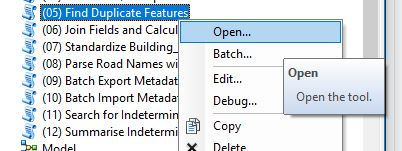
\includegraphics[width=2.09in,]{figures/delF-opentool} 

}

\caption{Opening the Delete Duplicate Features tool}\label{fig:delFopen}
\end{figure}

\subsection{Fill out the parameters}\label{fill-out-the-parameters-4}

Next, fill out the parameters for the tool. Here, we want to search all
Feature Classes within Feature Datasets in the Example.gdb for duplicate
features (Fig. \ref{fig:delFparams}). We specify that we want to keep
the default XY Tolerance and Z Tolerance parameters to zero, though this
could be increased to allow duplicate geometry checks to be more
lenient.

\begin{figure}[H]

{\centering 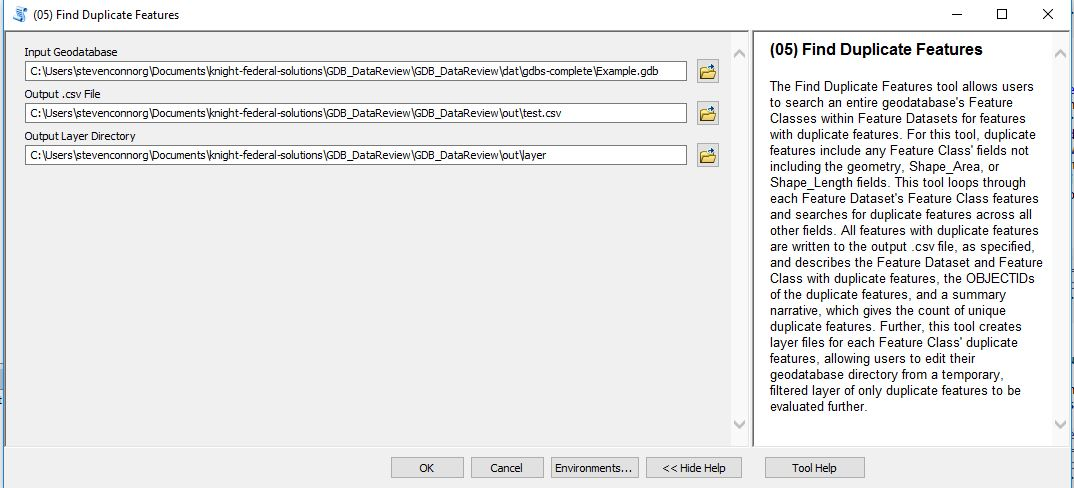
\includegraphics[width=0.8\linewidth,]{figures/delF-params} 

}

\caption{Delete Duplicate Features parameters}\label{fig:delFparams}
\end{figure}

\subsection{Run the Tool and View
Results}\label{run-the-tool-and-view-results-4}

While the tool runs (with Background Processing disabled), we can see
the messages from the tool, which displays how many duplicate features
will be deleted across each feature class, if applicable (Fig.
\ref{fig:delFmessages}). Here, we see that 102 duplicates were found in
the MilFlightTrack\_L feature class across 51 unique features,
indicating that each of the 51 features may have been duplicated once
(51 x 2 = 102).

\begin{figure}[H]

{\centering 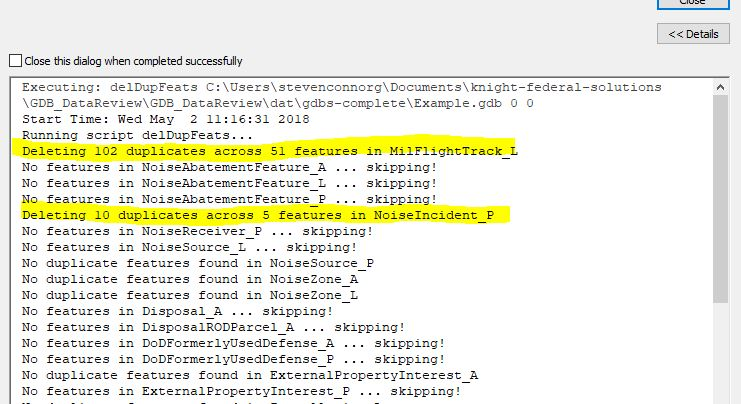
\includegraphics[width=3.86in,]{figures/delF-messages} 

}

\caption{Delete Duplicate Features messages}\label{fig:delFmessages}
\end{figure}

\hypertarget{chkGeom}{\chapter{Check and/or Repair
Geometries}\label{chkGeom}}

\section{Overview}\label{overview-5}

The Check and/or Repair Geometries tool allows users to search an entire
geodatabase's Feature Classes for geometry problems. This tool loops
through each Feature Dataset's Feature Class features and searches for
geometry problems, including null geometry, self intersections,
duplicate vertexes, and more.

If geometry problems exists, an output table is created containing the
following fields: CLASS, FEATURE\_ID, and PROBLEM. The feature classes
which contain geometry problems are then repaired.

After the repair is conducted, the subset of feature classes with
repaired geometry problems are checked again for geometry problems to
confirm their repair. Another output table is generated for the subset
of feature classes. An empty output table confirms the geometry problems
were correctly repaired.

\section{Parameters}\label{parameters-5}

The tool has 2 parameters:

\begin{enumerate}
\def\labelenumi{\arabic{enumi}.}
\tightlist
\item
  \textbf{Input\_Geodatabase (data type: Workspace)} - This parameter
  must be the path of the input geodatabase to search Feature Datasets'
  Feature Class features for duplicate features.
\item
  \textbf{Output\_Geodatabase (data type: Workspace)} - This parameter
  should be the path of the Installation Review Geodatabase to compile
  all CIP processing outputs in a single location.
\item
  \textbf{Repair Geometries? (data type: Boolean)} - Do you want to
  automatically repair geometries, where possible?
\item
  \textbf{Delete Null Geometries? (data type: Boolean)} - Do you want to
  automatically delete features that have null/empty geometries?
\end{enumerate}

\section{How to Use}\label{how-to-use-5}

\subsection{Begin by opening the
toolbox}\label{begin-by-opening-the-toolbox-5}

Navigate to the location of the script toolbox, then right-click the
`Check and/or Repair Geometry' script tool to open (Fig.
\ref{fig:chkGopen}).

\begin{figure}[H]

{\centering 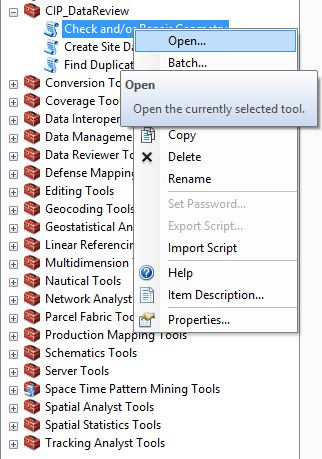
\includegraphics[width=1.68in,]{figures/chkG-open} 

}

\caption{Opening the Check and/or Repair Geometries tool}\label{fig:chkGopen}
\end{figure}

\subsection{Fill out the parameters}\label{fill-out-the-parameters-5}

Next, fill out the parameters for the tool. Here, we want to search all
Feature Classes within Feature Datasets in the Example.gdb for duplicate
features (Fig. \ref{fig:chkGparams}). Lastly, we specify where we want
to output the resulting tables, prefereably in an Installation Review
geodatabase specifically for holding CIP processing results.\\

\begin{figure}[H]

{\centering 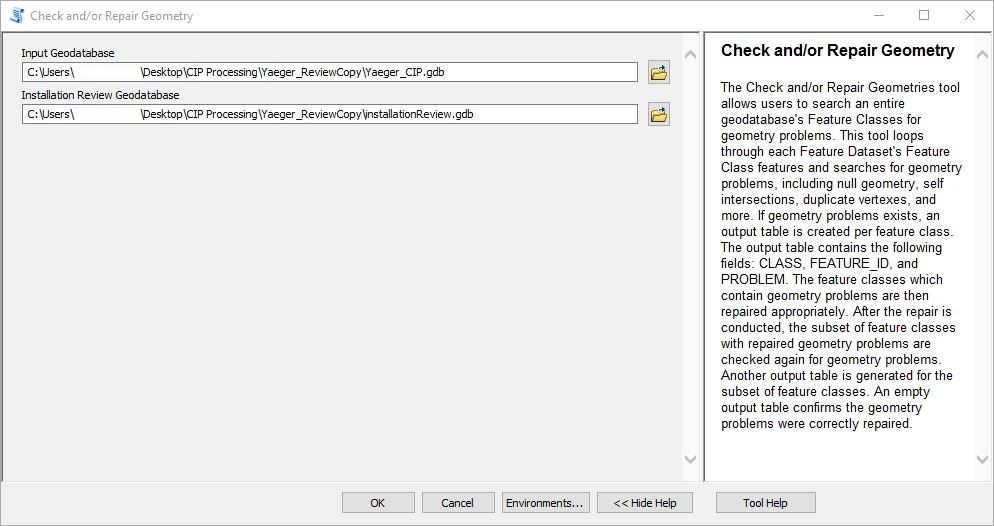
\includegraphics[width=4.05in,]{figures/chkG-params} 

}

\caption{Check and/or Repair Geometries tool parameters}\label{fig:chkGparams}
\end{figure}

\subsection{Run the Tool and View
Results}\label{run-the-tool-and-view-results-5}

While the tool runs (with Background Processing disabled), we can see
the messages from the tool, which displays the following: how many
feature classes are being checked for geometry problems, how many
geometry problems that were found, where the output results are found,
how many and which feature classes will be processed to repair geometry
problems, how many feature classes are being re-checked for geometry
errors, and how many geometry problems were found after the re-check
(Fig. \ref{fig:chkGmessages}).

\begin{figure}[H]

{\centering 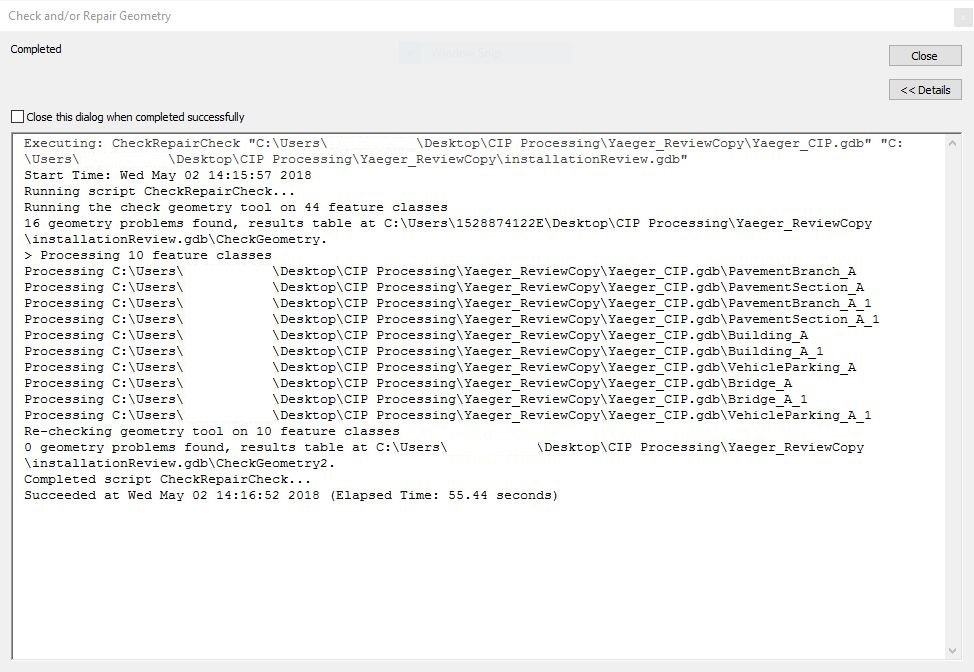
\includegraphics[width=5.07in,]{figures/chkG-messages} 

}

\caption{Output messages from the Check and/or Repair Geometries tool}\label{fig:chkGmessages}
\end{figure}

Here, we see that 16 geometry problems were found in the Yaeger CIP
geodatabase across 10 different feature classes, with each listed. A
re-check was conducted on the 10 feature classes and then 0 geometry
problems were found (Fig. \ref{fig:chkGafter}).

\begin{figure}[H]

{\centering 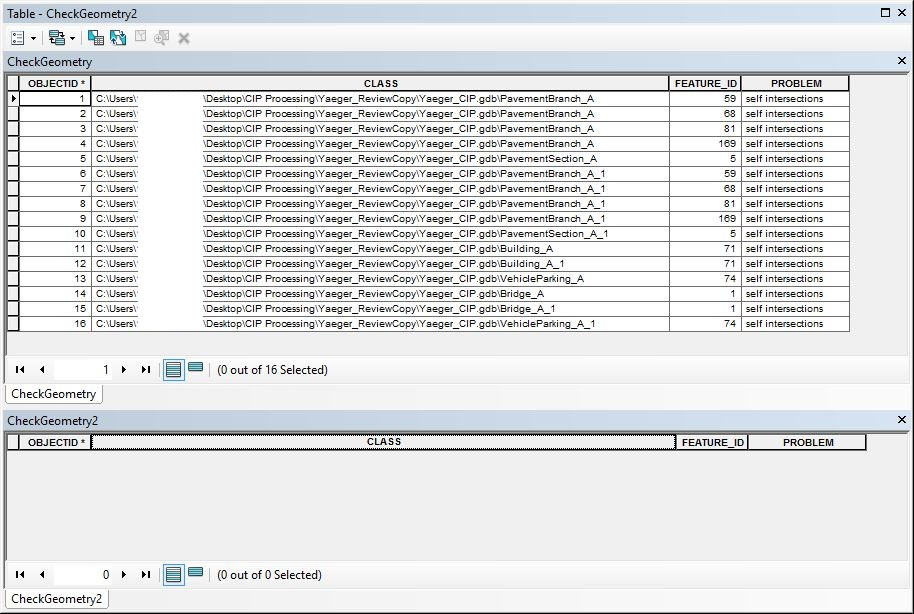
\includegraphics[width=4.76in,]{figures/chkG-after} 

}

\caption{Output table of duplicate geometries found for each Feature Class, with the re-run showing that all geometries have been fixed.}\label{fig:chkGafter}
\end{figure}

\hypertarget{stdAdd1}{\chapter{Standardize 1 Address
Field}\label{stdAdd1}}

\section{Overview}\label{overview-6}

The Standardize Address Field tool allows users to standardize 1 address
field in a feature class. This tool works by searching the address field
within the input feature class, then replaces any street prefixes (e.g.:
North, north, East, West) with a standard prefix abbreviation (i.e.:
``N'', ``S'', ``E'', and ``W''), while all suffixes (e.g.: AVE, Avenue,
Street) are reformatted to
\href{https://github.com/allanbreyes/udacity-data-science/blob/master/p2/data/suffixes.csv}{standard
USPS suffixes}.

\section{Parameters}\label{parameters-6}

The tool has 2 parameters:

\begin{enumerate}
\def\labelenumi{\arabic{enumi}.}
\tightlist
\item
  \textbf{Feature Class (data type: Feature Class )} - The path to the
  Feature Class with the address field to standardize.
\item
  \textbf{Field (data type: Field)} - The address field in the Feature
  Class to be standardized.
\end{enumerate}

\section{How to Use}\label{how-to-use-6}

\subsection{Begin by opening the
toolbox}\label{begin-by-opening-the-toolbox-6}

Navigate to the location of the script toolbox, then right-click the
`Standardize 1 Address Field' script tool to open (Fig.
\ref{fig:std1open}).

\begin{figure}[H]

{\centering 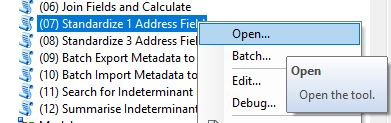
\includegraphics[width=2.04in,]{figures/std1-opentool} 

}

\caption{Opening the Standardize Address Field tool}\label{fig:std1open}
\end{figure}

\subsection{Fill out the parameters}\label{fill-out-the-parameters-6}

Next, fill out the parameters for the tool. Here, we want to update the
buildingAddress field in the Building\_A Feature Class in the
Example.gdb (Fig. \ref{fig:std1params}) because we notice none
standardized addresses in the field (Fig. \ref{fig:std1before}).

\begin{figure}[H]

{\centering 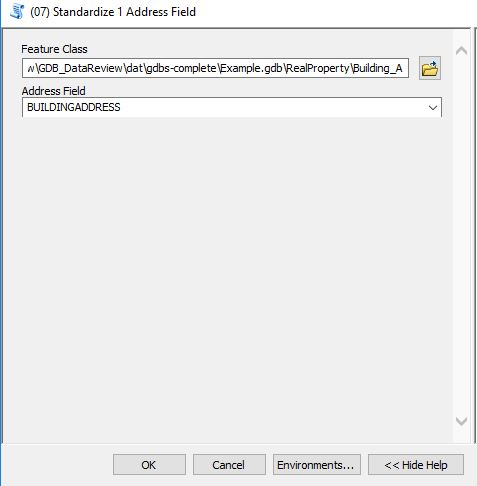
\includegraphics[width=2.48in,]{figures/std1-toolparams} 

}

\caption{Tool parameters to run}\label{fig:std1params}
\end{figure}\begin{figure}[H]

{\centering 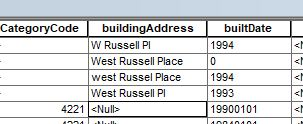
\includegraphics[width=1.06in,]{figures/std1-before} 

}

\caption{The unstandardized address field attributes before running the tool.}\label{fig:std1before}
\end{figure}

\subsection{Run the Tool and View
Results}\label{run-the-tool-and-view-results-6}

After the tool has run, we can see that the building address values have
been appropriately standardized (Fig. \ref{fig:std1after}).

\begin{figure}[H]

{\centering 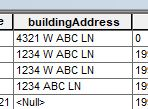
\includegraphics[width=0.77in,]{figures/std1-after} 

}

\caption{The standardized address field attributes after running the tool.}\label{fig:std1after}
\end{figure}

\hypertarget{std3}{\chapter{Standardized Road Prefix, Name, and
Suffix}\label{std3}}

\section{Overview}\label{overview-7}

The purpose of this tool is to standardize the 3 field (road prefix,
road name, and road suffix) values within a feature class. This tool
works by first searching the ROADNAME field within that feature class,
then removes any prefixes or suffixes within the field and moves them to
the appropriate field. For all prefixes and suffixes found, the prefixes
are reformatted to ``N'', ``S'', ``E'', and ``W.'' For all suffixes
found, the suffixes are reformatted to
\href{https://github.com/allanbreyes/udacity-data-science/blob/master/p2/data/suffixes.csv}{standard
USPS suffixes}.

\section{Parameters}\label{parameters-7}

The tool has 4 parameters:

\begin{enumerate}
\def\labelenumi{\arabic{enumi}.}
\tightlist
\item
  \textbf{Road Feature Class (data type: Feature Class)} - This
  parameter must be the path to the Feature Class that has the 3 road
  fields to be standardized.
\item
  \textbf{Prefix Field (data type: Field)} - The field within the
  feature class that has or should have road prefixes.
\item
  \textbf{Name Field (data type: Field)} - The field within the feature
  class that has road names.
\item
  \textbf{Suffix Field (data type: Field)} - The field within the
  feature class that has or should have road suffixes.
\end{enumerate}

\section{How to Use}\label{how-to-use-7}

\subsection{Begin by opening the
toolbox}\label{begin-by-opening-the-toolbox-7}

Navigate to the location of the script toolbox, then right-click the
`Standardize 3 Address Fields' script tool to open (Fig.
\ref{fig:std3open}).

\begin{figure}[H]

{\centering 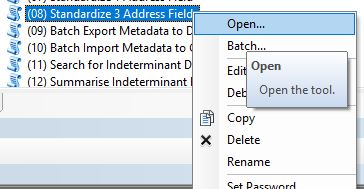
\includegraphics[width=1.9in,]{figures/std3-open} 

}

\caption{Opening Standardize Road Prefix, Name, and Suffix tool}\label{fig:std3open}
\end{figure}

\subsection{Fill out the parameters}\label{fill-out-the-parameters-7}

Next, fill out the parameters for the tool. Here, we want to update the
road prefix, road name, and road suffix fields in the RoadCenterline\_L
feature class (Fig. \ref{fig:std3params}). The fields can be derived
directly from the Feature Class by using the drop-down menu.

\begin{figure}[H]

{\centering 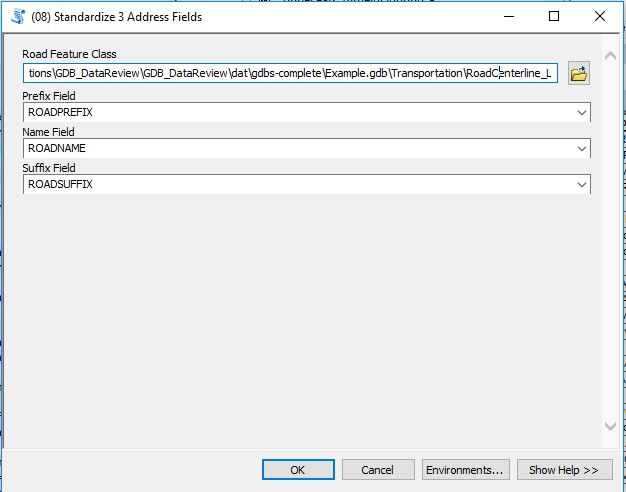
\includegraphics[width=3.26in,]{figures/std3-toolparams} 

}

\caption{Standardize Road Prefix, Name, and Suffix tool parameters}\label{fig:std3params}
\end{figure}

\section{Run the Tool and View
Results}\label{run-the-tool-and-view-results-7}

Before running the tool, we see that, indeed, the road prefixes and road
suffixes are incorrectly populated inside the road name field Open the
destinate Feature Class and view the update destination field values
(Fig. \ref{fig:std3before}).

\begin{figure}[H]

{\centering 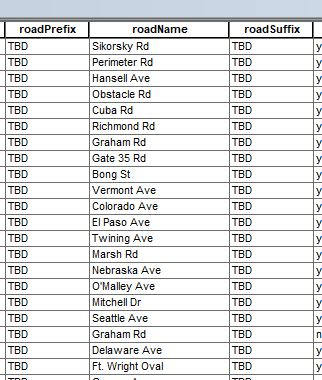
\includegraphics[width=1.68in,]{figures/std3-before} 

}

\caption{Unstandardized road prefixes, names, and suffixes before running the tool.}\label{fig:std3before}
\end{figure}

After running the tool, we can see that the prefixes and suffixes have
been populated in the correct fields, and have also been standardized to
match USPS standards (Fig. \ref{fig:std3after}).

\begin{figure}[H]

{\centering 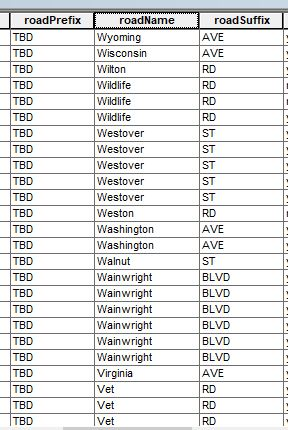
\includegraphics[width=1.5in,]{figures/std3-after} 

}

\caption{Standardized road prefixes, names, and suffixes after running the tool.}\label{fig:std3after}
\end{figure}

\hypertarget{indtSearch}{\chapter{Search for Missing and Indeterminant
Data}\label{indtSearch}}

\section{Overview}\label{overview-8}

Search a `source' geodatabase for indeterminate data from feature
dataset/feature class combinations in a target geodatabase. First,
searches for missing feature datasets in target geodatabase not in
source geodatabase. Then, searches for feature classes in `x' feature
dataset. Then, for each feature class in the source geodatabase, this
tool searches for `indeterminate' values in each field. Indeterminate
values, here, means any null, to be determined (TBD), or `other' values.

This tool creates 4 output tables, each prepended with the name of the
Model\_Geodatabase (e.g.: If your `model' geodatabase called `CIP', the
tables will be called (CIP\_MissingFDS, CIP\_Missing\_FCs,
CIP\_MissingFields, and CIP\_MissingData). These tables include:

\begin{itemize}
\tightlist
\item
  {[}modelGeodatabaseName{]}\_MissingFDS - Gives a list of Feature
  Datasets within the target geodatabase that are not included in the
  source geodatabase.\\
\item
  {[}modelGeodatabaseName{]}\_MissingFCs - Gives a list of Feature
  Classes for each Feature Dataset within the target geodatabase that
  are not included in the source geodatabase.\\
\item
  {[}modelGeodatabaseName{]}\_MissingFields - Gives a list of Fields for
  each Feature Dataset/Feature Class combination within the target
  geodatabase that are not included in the source geodatabase.\\
\item
  {[}modelGeodatabaseName{]}\_MissingData - For each Feature
  Dataset/Feature Class combination in both the target and source
  geodatabase, this table gives an overview of missing attributes for
  each field in the source geodatabase's Feature Class.

  \begin{itemize}
  \tightlist
  \item
    For Fields in each of the source geodatabase's Feature Classes, this
    table highlights fields not included in the target geodatabase's
    Feature Class under the `FIELD\_NONSDS' column (e.g.:
    `FIELD\_NONSDS' = F when fields are included in both geodatabases,
    and `FIELD\_NONSDS' = T when the field exists in the source
    geodatabase for said Feature Class, but not the target geodatabase's
    Feature Class).
  \item
    This table then lists whether or not the feature class is empty
    (i.e.: EMPTY\_FC = T or F).
  \item
    Then, for each field, the MissingData table gives a count of
    Null\footnote{Null values include :None, ``None'', ``none'',
      ``NONE'', ``'',``-99999'',``77777'',77777, "
      ``,''NA``,''na``,''N/A``,''n/a``,''NULL``,''Null``,''``,''null``,''``''``,''
      ``,'' ``,'' ``,'' ``}, `TBD'\footnote{TBD values include :
      ``tbd'',``TBD'',``To be determined'',``Tbd'',99999,``99999''}, and
    `Other'\footnote{Other values include : ``Other'', ``other'',
      ``OTHER'',``88888'',88888} features, further giving the counts of
    each value in `NULL\_VALUE\_COUNTS', `TBD\_VALUE\_COUNTS', and
    `OTHER\_VALUE\_COUNTS' fields.
  \item
    The sum of the Null, TBD, and Other features are populated in the
    `TOTAL\_INDT\_COUNT' (i.e.: Total indeterminant feature count), with
    the `TOTAL\_DET\_COUNT' column giving the total number of features
    with `determinated' values (i.e.: not indeterminant values).
  \item
    The POP\_VALS column lists the count of all unique populated values
    for each field, while the INC\_POP\_VALS column lists any field
    values that are not included in the field's domain.
  \end{itemize}
\end{itemize}

\section{Parameters}\label{parameters-8}

The tool has 2 parameters:

\begin{enumerate}
\def\labelenumi{\arabic{enumi}.}
\tightlist
\item
  \textbf{Source Geodatabase (data type: Workspace/File Geodatabase)} -
  The path to the file geodatabase to be searched for
  indeterminant/missing data.
\item
  \textbf{Target Geodatabase (data type: Workspace/File Geodatabase)} -
  The path to the file geodatabase with which the source geodatabase
  will be compared against.
\end{enumerate}

\BeginKnitrBlock{warnh1}
Disclaimer!
\EndKnitrBlock{warnh1} \BeginKnitrBlock{warnp}

This script tool currently requires an Advanced ArcGIS License!
\EndKnitrBlock{warnp}

\section{How to Use}\label{how-to-use-8}

\subsection{Begin by opening the
toolbox}\label{begin-by-opening-the-toolbox-8}

Navigate to the location of the script toolbox, then right-click the
`Search for Indeterminant Data' script tool to open (Fig.
\ref{fig:indtSearchopen}).

\begin{figure}[H]

{\centering 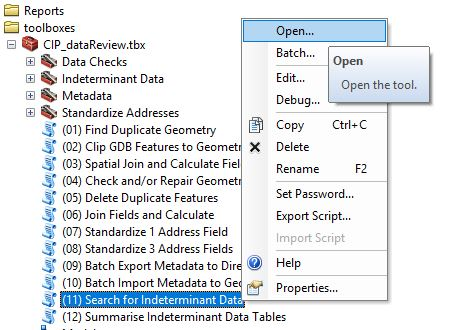
\includegraphics[width=2.39in,]{figures/indtSearch-open} 

}

\caption{Opening the Search for Missing and Indeterminant Data tool}\label{fig:indtSearchopen}
\end{figure}

\subsection{Fill out the parameters}\label{fill-out-the-parameters-8}

Next, fill out the parameters for the tool. Here, we want to compare the
`Example.gdb' against the `CIP.gdb' (Fig. \ref{fig:indtSearchparams}).
The fields can be derived directly from the Feature Class by using the
drop-down menu.

\begin{figure}[H]

{\centering 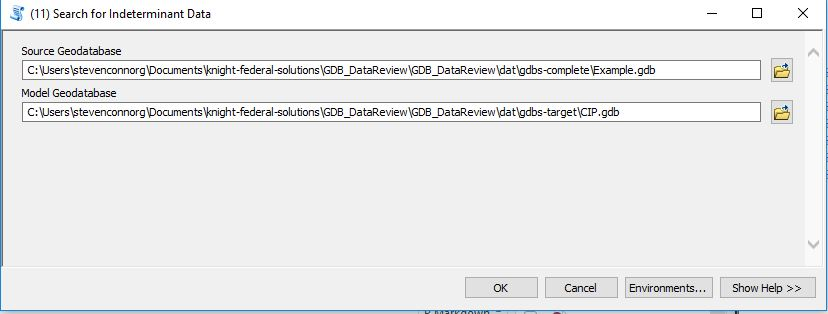
\includegraphics[width=4.31in,]{figures/indtSearch-params} 

}

\caption{Opening the Search for Missing and Indeterminant Data tool}\label{fig:indtSearchparams}
\end{figure}

\section{Run the Tool and View
Results}\label{run-the-tool-and-view-results-8}

While we run the tool, we can see view the messages of the tool, giving
a listing of the fields being searched for indeterminant data with the
counts of indeterminant values (Fig. \ref{fig:indtSearchmessages}).

\begin{figure}[H]

{\centering 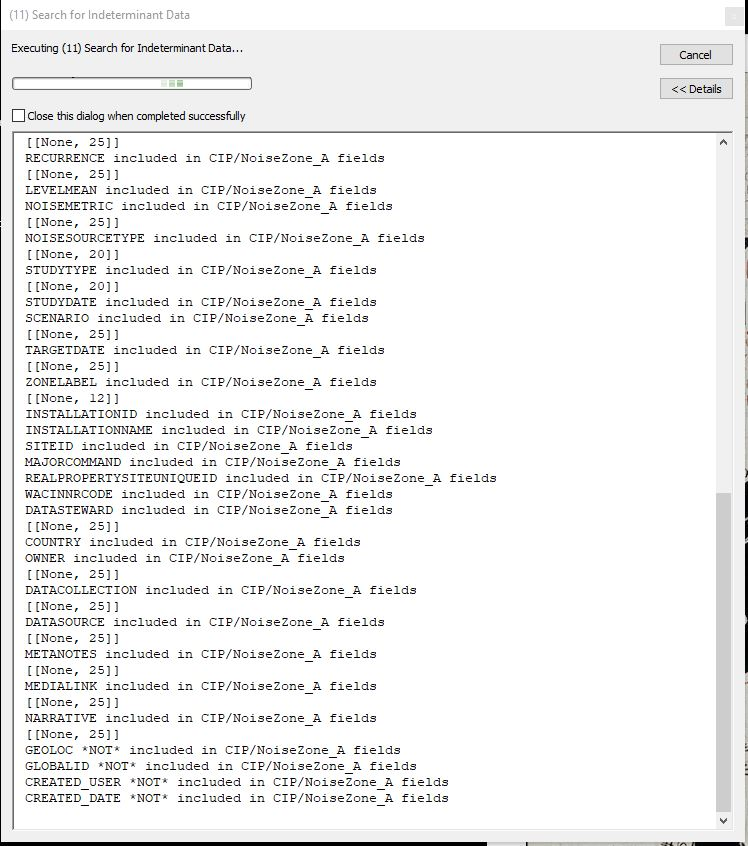
\includegraphics[width=3.9in,]{figures/indtSearch-messages} 

}

\caption{Search for Missing and Indeterminant Data tool messages}\label{fig:indtSearchmessages}
\end{figure}

After the tool has run, we can inspect the output tables within the
`Example.gdb' geodatabase (Fig. \ref{fig:indtSearchtables}). Opening the
CIP\_MissingFDS table, we see that the Example geodatabase have no
missing Feature Datasets \ref{fig:indtSearchmissingFDS}).

\begin{figure}[H]

{\centering 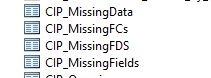
\includegraphics[width=1.1in,]{figures/indtSearch-tables} 

}

\caption{Search for Missing and Indeterminant Data output tables}\label{fig:indtSearchtables}
\end{figure}\begin{figure}[H]

{\centering 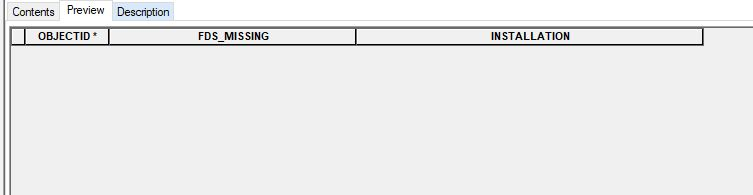
\includegraphics[width=3.92in,]{figures/indtSearch-missingFDS} 

}

\caption{The output Missing Feature Datasets table}\label{fig:indtSearchmissingFDS}
\end{figure}

Examining the MissingFCs table, we see that the Example geodatabase has
one Feature Class, RoadSeg\_L from the Transportation Feature Dataset,
missing when compared with the CIP geodatabase
\ref{fig:indtSearchmissingFCs}).

\begin{figure}[H]

{\centering 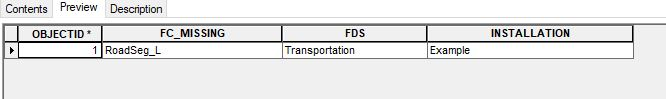
\includegraphics[width=3.47in,]{figures/indtSearch-missingFCs} 

}

\caption{The output Missing Feature Classes table}\label{fig:indtSearchmissingFCs}
\end{figure}

We can look at the MissingFLD table to see which fields are missing from
each Feature Class from the target geodatabase that are included in the
source geodatabase \ref{fig:indtSearchmissingFLDs}).

\begin{figure}[H]

{\centering 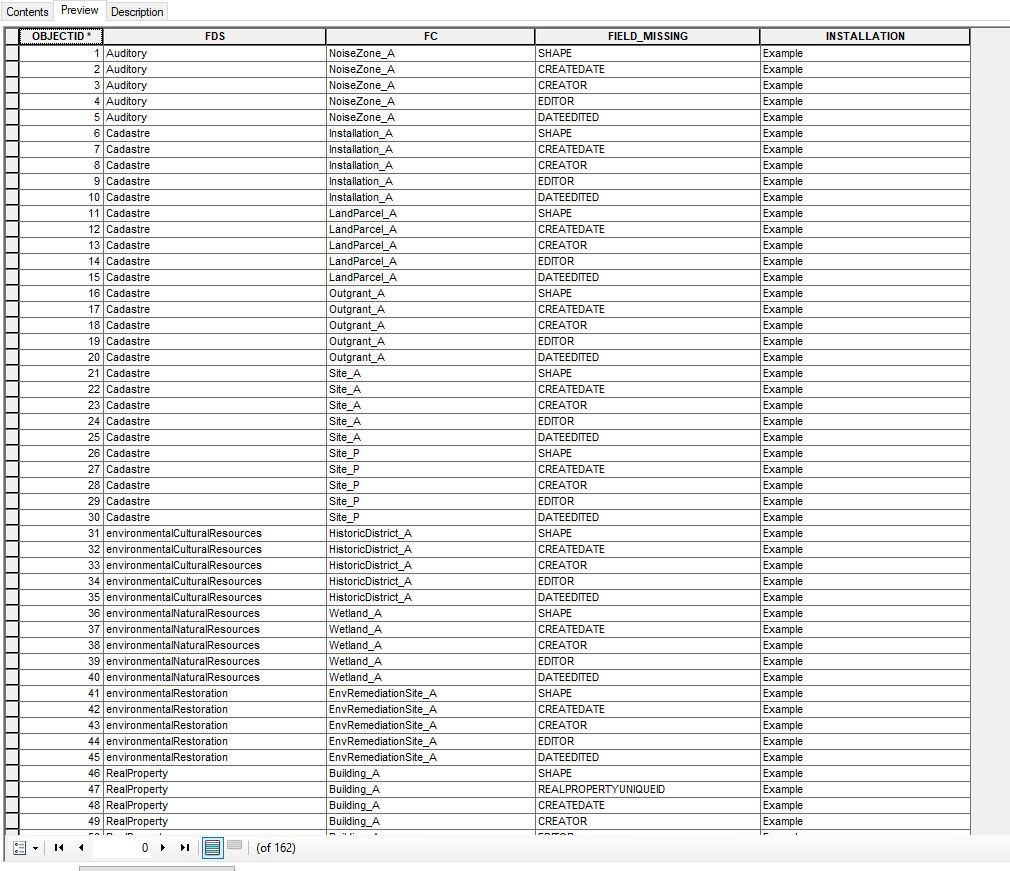
\includegraphics[width=5.26in,]{figures/indtSearch-missingFLDs} 

}

\caption{The output Missing Feature Fields table}\label{fig:indtSearchmissingFLDs}
\end{figure}

To examine indeterminant field attribution, we can examine the
MissingData table \ref{fig:indtSearchmissingData}).

\begin{figure}[H]

{\centering 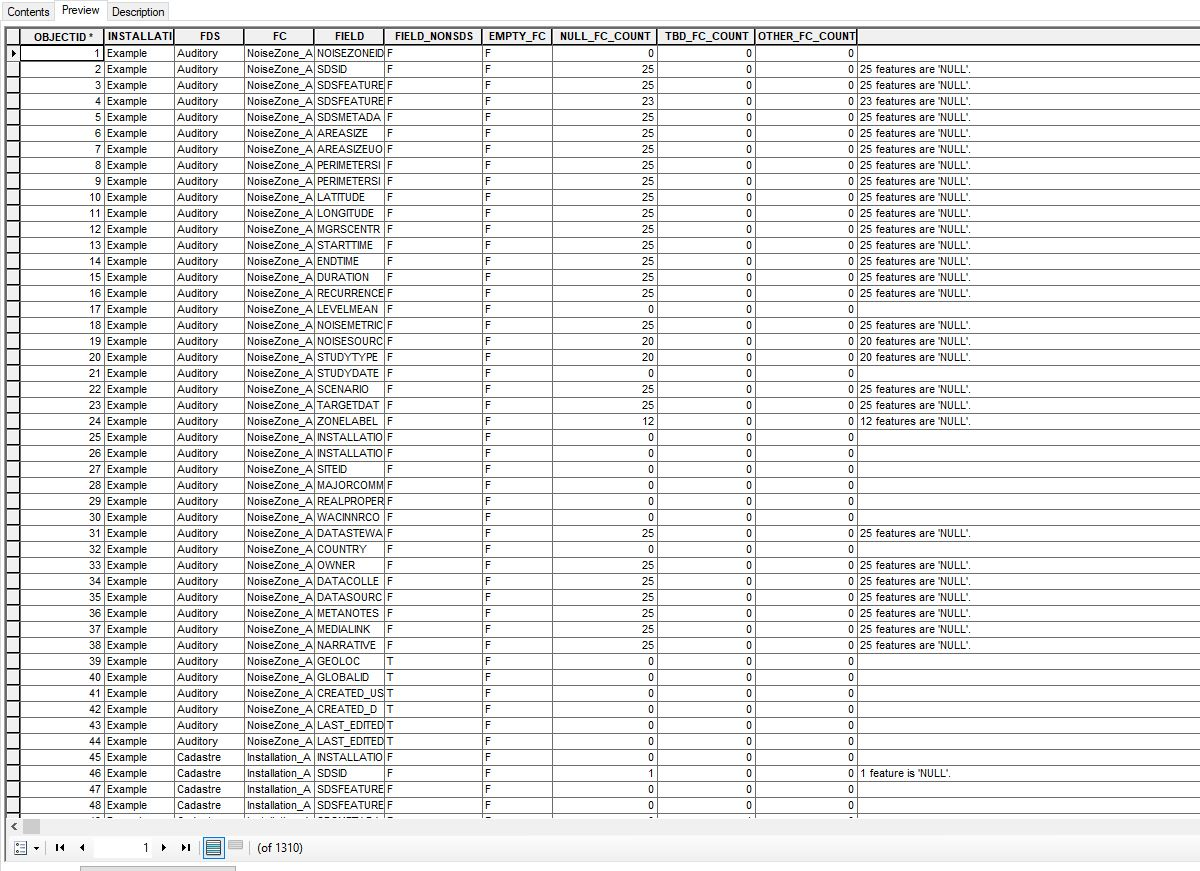
\includegraphics[width=6.25in,]{figures/indtSearch-missingData} 

}

\caption{The output Missing Data table}\label{fig:indtSearchmissingData}
\end{figure}

\hypertarget{summIndt}{\chapter{Summarise Indeterminant/Missing Data
Tables}\label{summIndt}}

\section{Overview}\label{overview-9}

This tool takes the 4 tables created with the
\protect\hyperlink{indtSearch}{Search for Missing and Indeterminant
Data} tool and creates an outbook Excel Workbook which includes the
following sheets:

\begin{enumerate}
\def\labelenumi{\arabic{enumi}.}
\tightlist
\item
  \textbf{Summary\_by\_FC} - gives the counts and percentages of
  `Other', `Null', and `TBD' cells by Feature Class, as well as the
  total counts and percentages of indeterminate (Other + Null + TBD) and
  determinate cells (not Other, Null, or TBD),
\item
  \textbf{Summary\_by\_Field} - gives the same statistics as the
  Summary\_by\_FC sheet, but broken down further by Feature Class
  Fields,
\item
  \textbf{Empty Feature Classes} - gives the standard Feature Classes in
  the comparison geodatabase not included in the input geodatabase(i.e.:
  Feature Classes included in comparison geodatabases)
\item
  \textbf{Indeterminate\_Overview}, gives :

  \begin{itemize}
  \tightlist
  \item
    The total count of feature classes that are empty
  \item
    The total number of standard feature classes that are empty
  \item
    The source geodatabase installation name
  \item
    The total number of missing feature classes
  \item
    The total number of missing feature datasets
  \item
    The total number of empty fields from empty feature classes
  \item
    The total number of empty fields from non-empty feature classes.
  \end{itemize}
\end{enumerate}

\section{Parameters}\label{parameters-9}

The inputs required for this tool to work are the 4 output tables
created with the ``Search for Indeterminate Data'' script tool from one
comparison geodatabase (\textbf{repeat:} ensure these are all from the
same comparison geodatabase {[}i.e.: {[}comparison GDB{]} is the same
across all four input tables{]}):

\begin{enumerate}
\def\labelenumi{\arabic{enumi}.}
\tightlist
\item
  \textbf{comparisonGDBname\_MissingFDS Table (data type: GDB Table)} -
  The path to the MissingFDS table created with the
  \protect\hyperlink{indtSearch}{Search for Missing and Indeterminant
  Data} tool for one `target' geodatabase.
\item
  \textbf{comparisonGDBname\_MissingFCs (data type: GDB Table)} - The
  path to the MissingFCs table created with the
  \protect\hyperlink{indtSearch}{Search for Missing and Indeterminant
  Data} tool for one `target' geodatabase.
\item
  \textbf{comparisonGDBname\_MissingFields (data type: GDB Table)} - The
  path to the MissingFields table created with the
  \protect\hyperlink{indtSearch}{Search for Missing and Indeterminant
  Data} tool for one `target' geodatabase.
\item
  \textbf{comparisonGDBname\_MissingData (data type: GDB Table)} - The
  path to the MissingData table created with the
  \protect\hyperlink{indtSearch}{Search for Missing and Indeterminant
  Data} tool for one `target' geodatabase.
\item
  \textbf{Output Excel File' (data type: .xlsx file)} - The path to the
  output Excel Workbook to save the summary sheets to.
\end{enumerate}

\BeginKnitrBlock{warnh1}
Disclaimer!
\EndKnitrBlock{warnh1} \BeginKnitrBlock{warnp}

This script tool requires a few non-standard ArcGIS 10.x Python modules:
\href{http://www.numpy.org/}{numpy} and
\href{https://pandas.pydata.org/}{pandas}. To install these modules for
use in ArcGIS, you can download and install the modules using the
commands ``pip install pandas'' and ``pip install numpy.''

To do this, follow these instructions:

\begin{enumerate}
\def\labelenumi{\arabic{enumi}.}
\tightlist
\item
  Press the windows key on your keyboard
\item
  Type ``cmd'' to open the command prompt window
\item
  Set your working directory to the ArcGIS Python directory with the
  `pip' command (e.g.: if you are running ArcMap10.6, input:
  ``C:/Python27/ArcGIS10.6/Scripts'')
\item
  Type `pip install numpy' and press enter, then type `pip install
  pandas' and press enter. If all goes well, you will have these modules
  successfully installed for use in ArcGIS' Python distribution
\end{enumerate}
\EndKnitrBlock{warnp}

\section{How to Use}\label{how-to-use-9}

\subsection{Begin by opening the
toolbox}\label{begin-by-opening-the-toolbox-9}

Navigate to the location of the script toolbox, then right-click the
`Summarise Indeterminant Data Tables' script tool to open (Fig.
\ref{fig:summIndtopen}).

\begin{figure}[H]

{\centering 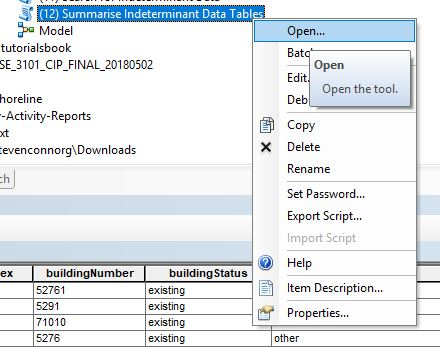
\includegraphics[width=2.29in,]{figures/summIndt-open} 

}

\caption{Opening the Summarise Indeterminant Data Tables tool}\label{fig:summIndtopen}
\end{figure}

\subsection{Fill out the parameters}\label{fill-out-the-parameters-9}

Next, fill out the parameters for the tool. Here, we want to summarise
the Indeterminant Data Tables created in the Example.gdb that was
created when comparing against the CIP geodatabase. Again, be sure that
these input tables all derive from the same target geodatabase!

\begin{figure}[H]

{\centering 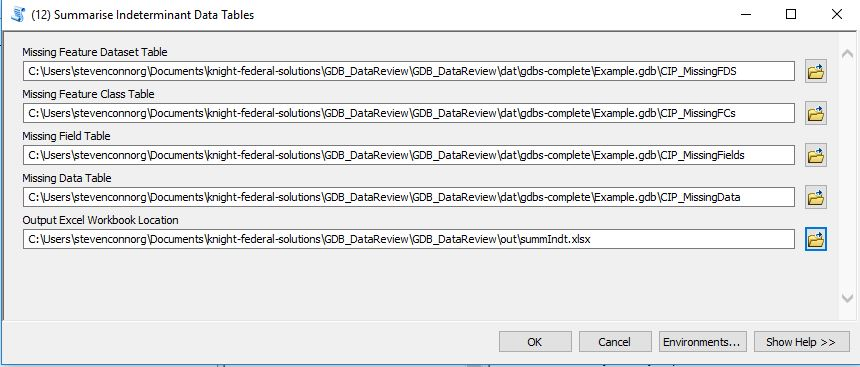
\includegraphics[width=4.48in,]{figures/summIndt-toolparams} 

}

\caption{Setting the parameters for the Summarise Indeterminant Data Tables tool }\label{fig:summIndtparams}
\end{figure}

\section{Run the Tool and View
Results}\label{run-the-tool-and-view-results-9}

While we run the tool, we can see view the messages of the tool (Fig.
\ref{fig:summIndtmessages}).

\begin{figure}[H]

{\centering 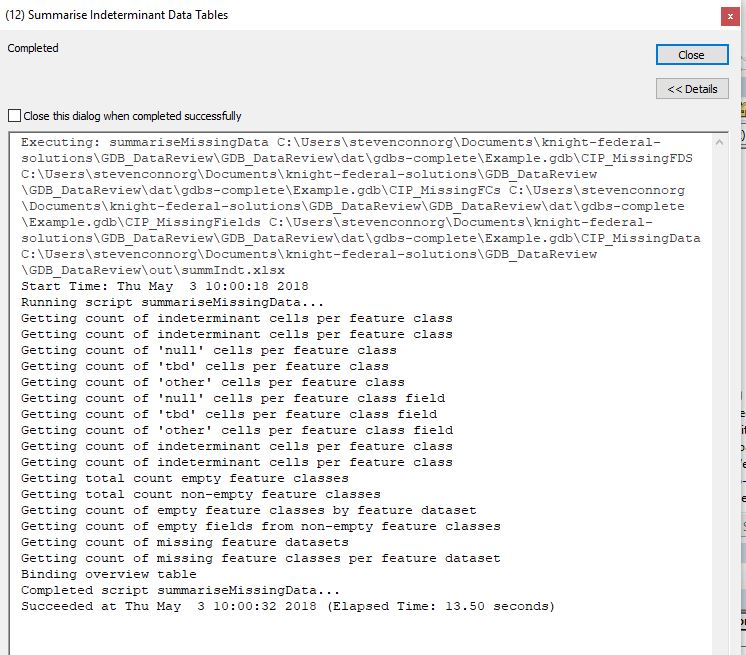
\includegraphics[width=3.89in,]{figures/summIndt-messages} 

}

\caption{Opening the Delete Duplicate Features tool}\label{fig:summIndtmessages}
\end{figure}

After the tool has run, we can open the output Excel Workbook we
specified to see the 4 output sheets : Summary\_by\_FC,
Summary\_by\_Field, Empty Feature Classes, and Indeterminate\_Overview
(Fig. \ref{fig:summIndtsheets}).

\begin{figure}[H]

{\centering 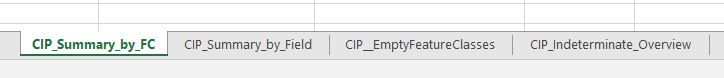
\includegraphics[width=3.77in,]{figures/summIndt-sheets} 

}

\caption{The output Excel Workbook sheets Summary by FC, Summary by Field, Empty Feature Classes, and Indeterminate Overview}\label{fig:summIndtsheets}
\end{figure}

Viewing the Summary\_by\_FC sheets gives us a comprehensive overview of
the counts and percentages of indeterminant Attribute Table cells by
indeterminant data type (i.e.: Null, TBD, and Other) (Fig.
\ref{fig:summIndtsheet1}).

\begin{figure}[H]

{\centering \includegraphics[width=9.41in,]{figures/summIndt-sheet1} 

}

\caption{The output Summary by Feature Class table}\label{fig:summIndtsheet1}
\end{figure}

The Summary\_by\_Field provides provides a breaks down of the
Summary\_by\_FC table by field (Fig. \ref{fig:summIndtsheet2}).

\begin{figure}[H]

{\centering \includegraphics[width=8.36in,]{figures/summIndt-sheet2} 

}

\caption{The output Summary by Field table}\label{fig:summIndtsheet2}
\end{figure}

The Empty Feature Classes sheet provides a listing of the Feature
Classes included in the Example.gdb that are empty, as well as the empty
fields from those empty feature classes (Fig. \ref{fig:summIndtsheet3}).

\begin{figure}[H]

{\centering \includegraphics[width=3.67in,]{figures/summIndt-sheet3} 

}

\caption{The output Empty Feature Classes table}\label{fig:summIndtsheet3}
\end{figure}

Lastly, the Indeterminate\_Overview sheet provides a general overview of
missing and indeterminant data at a geodatabase level (Fig.
\ref{fig:summIndtsheet4}).

\begin{figure}[H]

{\centering \includegraphics[width=5.67in,]{figures/summIndt-sheet4} 

}

\caption{The output Indeterminate Overview table}\label{fig:summIndtsheet4}
\end{figure}

\hypertarget{exMeta}{\chapter{Batch Export Metadata}\label{exMeta}}

\section{Overview}\label{overview-10}

This tool provides an automated method to export metadata for each
Feature Dataset and Feature Class (within Feature Datasets) in the input
geodatabase, by exporting each item's metadata to an .xml file to an
output directory, as specified. This tool allows you to specify a
metadata translator. Within the scope of the Department of Defense
Instruction (DoDI) 8130.01, it is recommended that you download and
install the SDSFIE-M Metadata Style for ArcGIS from
\href{https://www.sdsfieonline.org/Standards/Metadata}{The Spatial Data
Standards for Facilities, Infrastructure, and Environment (SDSFIE)
Metadata standard}. In this case, you would change the input the
metadata translator to the ARCGIS2SDSFIE-M.xml\footnote{Under standard
  Windows installations, this should be located at ``C:/Program Files
  (x86)/ArcGIS/Desktop10.6/Metadata/Translator/ARCGIS2SDSFIE-M.xml''.}
provided with the SDSFIE-M Metadata Style for ArcGIS software.\^{}{[}Be
sure to install the software to the software path for your ArcGIS
distribution currently installed to view this metadata style within
ArcCatalog, for example: ``C:/Program Files (x86)/ArcGIS/Desktop10.X/''

If the source metadata is a Feature Dataset, the output .xml file is
named after the Feature Dataset. Alternatively, the output .xml metadata
for Feature Classes are exported with the Feature Dataset name prepended
before the Feature Class name.

These output .xml files can more easily be edited in batch using the
\href{http://insideidaho.org/helpdocs/batch_metadata_modifier_tool.html}{Batch
Metadata Modifier Tool} developed out of the University of Idaho's
Interactive Numeric \& Spatial Information Data Engine (INSIDE)
geospatial data clearinghouse.

\section{Parameters}\label{parameters-10}

The tool has 3 parameters:

\begin{enumerate}
\def\labelenumi{\arabic{enumi}.}
\tightlist
\item
  \textbf{Input Geodatabase (data type: Workspace/File Geodatabase)} -
  The input geodatabase to export Feature Dataset/Feature Class metadata
  from.
\item
  \textbf{Metadata Translator (data type: .XML file)} - The metadata
  translator to be used to create output .xml metadata files. These
  files are typically located at ``C:/Program Files
  (x86)/ArcGIS/{[}Desktop10.x{]}/Metadata/Translator/. Please change
  according to your ArcGIS installation file path.
\item
  \textbf{Output Directory (data type: Folder)} - The folder within
  which to write output .xml metadata files.
\end{enumerate}

\section{How to Use}\label{how-to-use-10}

\subsection{Begin by opening the
toolbox}\label{begin-by-opening-the-toolbox-10}

Navigate to the location of the script toolbox, then right-click the
`Batch Export Metadata to Directory' script tool to open (Fig.
\ref{fig:exMetaopen}).

\begin{figure}[H]

{\centering \includegraphics[width=2.23in,]{figures/exMeta-open} 

}

\caption{Opening the Batch Export Metadata tool}\label{fig:exMetaopen}
\end{figure}

\subsection{Fill out the parameters}\label{fill-out-the-parameters-10}

Next, fill out the parameters for the tool. Here, we want to export
metadata for all Feature Datasets and all Feature Classes (within those
Feature Datasets) within the Example.gdb geodatabase using the default
ARCGIS2FGDC metadata translator that comes with ArcGIS to a new
directory called `metadata' (Fig. \ref{fig:exMetaparams}).

\begin{figure}[H]

{\centering \includegraphics[width=4.49in,]{figures/exMeta-params} 

}

\caption{Batch Export Metadata tool parameters}\label{fig:exMetaparams}
\end{figure}

\section{Run the Tool and View
Results}\label{run-the-tool-and-view-results-10}

After running the tool, we can view the output metadata files inside the
output directory specified (Fig. \ref{fig:exMetaafter}). For Feature
Classes, the output .xml files has the associated Feature Dataset name
prepended to the filename, while Feature Dataset metadata file is simply
the name of the Feature Dataset.

\begin{figure}[H]

{\centering \includegraphics[width=3.93in,]{figures/exMeta-after} 

}

\caption{Batch Export Metadata output .xml files for each Feature Dataset/Feature Class}\label{fig:exMetaafter}
\end{figure}

\hypertarget{imMeta}{\chapter{Batch Import Metadata}\label{imMeta}}

\section{Overview}\label{overview-11}

This tool provides an automated method to import metadata for each
Feature Dataset and Feature Class (within Feature Datasets) in the input
geodatabase, following the output .xml file naming convention created
with the \protect\hyperlink{exMeta}{Batch Export Metadata} tool, and
potentially updated using the
\href{http://insideidaho.org/helpdocs/batch_metadata_modifier_tool.html}{Batch
Metadata Modifier Tool} developed out of the University of Idaho's
Interactive Numeric \& Spatial Information Data Engine (INSIDE)
geospatial data clearinghouse. As per SDSFIE standards, it is
recommended that you view this metadata using the
\href{https://www.sdsfieonline.org/Standards/Metadata}{SDSFIE-M Metadata
Style for ArcGIS}\footnote{When installing this tool, be sure to install
  it to the location of your current ArcGIS distribution on your
  computer, typically located at C:/Program Files
  (x86)/ArcGIS/Desktop10.6/, replacing with the approproate ArcGIS
  version}.

Alternatively, if you wish to import metadata from Feature Classes in a
Esri geodatabase, you should use the \protect\hyperlink{imMetaGDB}{Batch
Import Metadata from GDB} tool.

\section{Parameters}\label{parameters-11}

The tool has 2 parameters\footnote{More information may be found on the
  help page for ArcMap's
  \href{http://desktop.arcgis.com/en/arcmap/latest/tools/conversion-toolbox/metadata-importer.htm}{Metadata
  Importer}.}:

\begin{enumerate}
\def\labelenumi{\arabic{enumi}.}
\tightlist
\item
  \textbf{Input Geodatabase (data type: Workspace/File Geodatabase)} -
  The input geodatabase to export Feature Dataset/Feature Class metadata
  from.
\item
  \textbf{Input Metadata Directory (data type: Folder)} - The folder
  with the .xml files to import into the geodatabase features.
\end{enumerate}

\section{How to Use}\label{how-to-use-11}

\subsection{Begin by opening the
toolbox}\label{begin-by-opening-the-toolbox-11}

Navigate to the location of the script toolbox, then right-click the
`Batch Import Metadata' script tool to open (Fig. \ref{fig:imMetaopen}).

\begin{figure}[H]

{\centering \includegraphics[width=2.74in,]{figures/imMeta-open} 

}

\caption{Opening the Batch Import Metadata tool}\label{fig:imMetaopen}
\end{figure}

\subsection{Fill out the parameters}\label{fill-out-the-parameters-11}

Next, fill out the parameters for the tool. Here, we want to export
metadata for all Feature Datasets and all Feature Classes (within those
Feature Datasets) within the Example.gdb geodatabase using the default
ARCGIS2FGDC metadata translator that comes with ArcGIS to a new
directory called `metadata' (Fig. \ref{fig:imMetaparams}).

\begin{figure}[H]

{\centering \includegraphics[width=3.84in,]{figures/imMeta-params} 

}

\caption{Batch Import Metadata tool parameters}\label{fig:imMetaparams}
\end{figure}

\section{Run the Tool and View
Results}\label{run-the-tool-and-view-results-11}

While the tool runs, we can see which .xml files are being imported to
each Feature Dataset's/Feature Class' metadata, as well as which Feature
Datasets/Feature Classes do not have matching .xml files in the output
directory (Fig. \ref{fig:imMetamessages}).

\begin{figure}[H]

{\centering \includegraphics[width=3.89in,]{figures/imMeta-messages} 

}

\caption{Batch Import Metadata tool messages}\label{fig:imMetamessages}
\end{figure}

After running the tool, we can view the update Item Descriptions for the
Feature Classes and Feature Datasets imported with the .xml files (Fig.
\ref{fig:imMetaafter}). You can also change the way ArcMap displays the
metadata by going to Customize \textgreater{} ArcMap Options in ArcMap,
then clicking the Metadata tab and changing the Metadata Style in the
drop-down menu. You can find more information on Item Descriptions on
Esri's
\href{http://desktop.arcgis.com/en/arcmap/latest/map/working-with-arcmap/documenting-items-in-the-catalog-window.htm}{Item
Desecription Help Page}.

\begin{figure}[H]

{\centering \includegraphics[width=2.27in,]{figures/imMeta-after} 

}

\caption{Opening the Item Description to view updated Metadata}\label{fig:imMetaafter}
\end{figure}

\hypertarget{imMetaGDB}{\chapter{Batch Import Metadata from
GDB}\label{imMetaGDB}}

\section{Overview}\label{overview-12}

This tool provides an automated method to import metadata for each
Feature Dataset and Feature Class (within Feature Datasets) in the input
geodatabase from a source geodatabase. This tool different from the
\protect\hyperlink{imMeta}{Batch Import Metadata} tool because it
imports metadata from a source geodatabase and not from a directory of
metadata .xml files.

\section{Parameters}\label{parameters-12}

The tool has 3 parameters\footnote{More information of the Import Type
  and Auto Update parameters may be found at the help page for ArcMap's
  \href{http://desktop.arcgis.com/en/arcmap/latest/tools/conversion-toolbox/import-metadata.htm}{Import
  Metadata Tool}.}:

\begin{enumerate}
\def\labelenumi{\arabic{enumi}.}
\tightlist
\item
  \textbf{Source Geodatabase (data type: Workspace/File Geodatabase)} -
  The input geodatabase to export Feature Dataset/Feature Class metadata
  from.
\item
  \textbf{Target Geodatabase (data type: Workspace/File Geodatabase)} -
  The geodatabase to input metadata from the Source Geodatabase from.
\item
  \textbf{Sync Type (data type: String)} - How would you like the
  metadata items to be Syncronized upon import?\footnote{More
    information on Sync Type paramters may be found at the help file for
    the
    \href{http://desktop.arcgis.com/en/arcmap/latest/tools/conversion-toolbox/synchronize-metadata.htm}{Synchronize
    Metadata function}}

  \begin{itemize}
  \tightlist
  \item
    \emph{ALWAYS} --- Properties of the source item are always added to
    or updated in its metadata. Metadata will be created if it doesn't
    already exist. This is the deault.
  \item
    \emph{ACCESSED} --- Properties of the source item are added to or
    updated in its metadata when it is accessed. Metadata will be
    created if it doesn't already exist.
  \item
    \emph{CREATED} --- Metadata will be created and properties of the
    source item will be added to it if the item doesn't already have
    metadata.
  \item
    \emph{NOT\_CREATED} --- Properties of the source item are added to
    or updated in existing metadata.
  \item
    \emph{OVERWRITE} --- The same as ``ALWAYS'' except all information
    that can be recorded automatically in the metadata will be recorded.
    Any properties typed in by a person will be replaced with the item's
    actual properties.
  \item
    \emph{SELECTIVE} --- The same as ``OVERWRITE'' except the title and
    the content type will not be overwritten with default values for the
    item. Used when metadata is upgraded to the ArcGIS 10.x metadata
    format.
  \end{itemize}
\end{enumerate}

\section{How to Use}\label{how-to-use-12}

\subsection{Begin by opening the
toolbox}\label{begin-by-opening-the-toolbox-12}

Navigate to the location of the script toolbox, then right-click the
`Batch Import Metadata to Geodatabase from GDB' script tool to open
(Fig. \ref{fig:imMetaopen}).

\begin{figure}[H]

{\centering \includegraphics[width=2.69in,]{figures/imMetaArc-open} 

}

\caption{Opening the Batch Import Metadata tool}\label{fig:imMetaArcopen}
\end{figure}

\subsection{Fill out the parameters}\label{fill-out-the-parameters-12}

Next, fill out the parameters for the tool. Here, we want to import
metadata from the geodatabas with metadata to the geodatabase without
metadata.

\begin{figure}[H]

{\centering \includegraphics[width=4.79in,]{figures/imMetaArc-params} 

}

\caption{Batch Import Metadata tool parameters}\label{fig:imMetaArcparams}
\end{figure}

\section{Run the Tool and View
Results}\label{run-the-tool-and-view-results-12}

While the tool runs, we can see which geodatabase Feature
Datasets/Feature Classes are being imported to each Feature
Dataset's/Feature Class' metadata, as well as which Feature
Datasets/Feature Classes do not have matching .xml files in the source
geodatabase (Fig. \ref{fig:imMetaArcmessages}).

\begin{figure}[H]

{\centering \includegraphics[width=3.89in,]{figures/imMetaArc-messages} 

}

\caption{Batch Import Metadata tool messages}\label{fig:imMetaArcmessages}
\end{figure}

After running the tool, we can view the update Item Descriptions for the
Feature Classes and Feature Datasets imported from the source
geodatabase (Fig. \ref{fig:imMetaArcafter}). If importing SDSFIE-M
metadata, it is recommended that you alter the way ArcMap displays the
metadata by going to Customize \textgreater{} ArcMap Options in ArcMap,
then clicking the Metadata tab and changing the Metadata Style in the
drop-down menu. To do this, you must view this metadata using the
\href{https://www.sdsfieonline.org/Standards/Metadata}{SDSFIE-M Metadata
Style for ArcGIS}\footnote{When installing this tool, be sure to install
  it to the location of your current ArcGIS distribution on your
  computer, typically located at C:/Program Files
  (x86)/ArcGIS/Desktop10.6/, replacing with the approproate ArcGIS
  version}. After doing this, we can view the SDSFIE-M metadata style
within ArcCatalog.

You can find more information on Item Descriptions on Esri's
\href{http://desktop.arcgis.com/en/arcmap/latest/map/working-with-arcmap/documenting-items-in-the-catalog-window.htm}{Item
Desecription Help Page}.

\begin{figure}[H]

{\centering \includegraphics[width=7.86in,]{figures/imMetaArc-after} 

}

\caption{Opening the Item Description to view updated Metadata}\label{fig:imMetaArcafter}
\end{figure}

\bibliography{packages.bib}


\end{document}
